\documentclass{article}
\usepackage{longtable}
\usepackage{indentfirst} 
\usepackage{amsmath,amssymb,bm}
%\usepackage{color}
%\usepackage{graphicx}
\usepackage{multicol}
\usepackage{here}
\usepackage[dvipdfmx]{hyperref}
\usepackage{pxjahyper}
\hypersetup{% hyperref 
 setpagesize=false,
 bookmarksnumbered=true,%
 bookmarksopen=true,%
 colorlinks=true,%
 linkcolor=blue,
 citecolor=red,
}
\usepackage[dvipdfm]{graphicx,color}

\newcommand{\tr}[1]{\textcolor{red}{#1}}
\newcommand{\tb}[1]{\textcolor{blue}{#1}}

\addtolength{\oddsidemargin}{-15mm}
\addtolength{\evensidemargin}{-15mm}
\addtolength{\textwidth}{30mm}
\addtolength{\topmargin}{-15mm}
\addtolength{\textheight}{30mm}

\title{\huge RESPACK Manual}
\author{\Large Kazuma Nakamura \\ (Department of Basic Sciences,
Kyushu Institute of Technology)}

\begin{document}
\maketitle
\begin{figure}[h] 
\centering

\includegraphics[width=8cm]{respack.eps}
\label{title}
\end{figure}

\clearpage 

\tableofcontents

\clearpage 

\section{Introduction}

\subsection{Program}

{\sc RESPACK} is a first-principles calculation software for evaluating the interaction parameters of materials, and is able to calculate the maximally localized Wannier functions, the RPA response functions, and frequency-dependent electronic interaction parameters. {\sc RESPACK} consists of three programs:
\begin{enumerate}
\item Wannier function calculation (\verb+wannier+),
\item dielectric function calculation (\verb+chiqw+),
\item electronic interaction calculation (direct integral: \verb+calc_w3d+, exchange integral: \verb+calcj3d+).
\end{enumerate}
These three programs are independent and each program needs
\begin{itemize}
\item input file (namelist form)
\item files as band-calculation output
\end{itemize}
{\sc RESPACK} receives input data from a band calculation using norm-conserving pseudopotentials with plane-wave basis sets. Automatic generation scripts which convert results of the band calculation to inputs for RESPACK are prepared for {\sc xTAPP} and {\sc Quantum ESPRESSO} codes. RESPACK can be successfully applied to wide materials such as metals, semiconductors, transition-metal compounds, and organic compounds. It supports {\sc OpenMP/MPI} and can be used in both laboratory-computer environment and System B at Institute for Solid State Physics, the University of Tokyo.

In this manual, we describe procedures to evaluate effective interaction parameters of Al as a benchmark. We also describe procedures of the case of La$_2$CuO$_4$ for constrained RPA calculation. Examples of Si, TiO$_2$, SrVO$_3$, organic compound (TMTSF)$_2$PF$_6$ are also presented.

\subsection{Unit system}

Programs are described in atomic units, but for input and output, \AA, \verb+Ry+, \verb+eV+, and lattice coordinates are used.

\subsection{Download source code}
The source code cab be downloaded from the official website https://sites.google.com/view/kazuma7k6r. Please download \verb+RESPACK.tar.gz+.

\subsection{\label{compile}Compiling source code}

Firstly, you unpack the source code \verb+RESPACK.tar.gz+ in your machine. In a directory \verb+RESPACK+, you see five directories (i) \verb+sample+ containing the inputs of calculation examples, (ii) \verb+src+ containing source codes, (iii) \verb+util+ containing necessary scripts to supplement calculation, 
\tr{(iv) {\tt config} containing setting files of {\tt CMake}}, and (iv) {\tt GPL} containing the software license. 

\subsubsection{\tr{Compile using CMake}}
\tr{RESPACK can be compiled using {\tt CMake}. In {\tt CMake}, user generates a working directory for compilation, and then creates a {\tt Makefile} script using the {\tt cmake} command. Then, the program is compiled using the {\tt make} command. The following is the work flow.}
\vspace{3mm}\hrule
\begin{verbatim}
tar -zxvf RESPACK.tar.gz
cd RESPACK
mkdir build
cd build
cmake -DCONFIG=gcc -DCMAKE_INSTALL_PREFIX=PATH_TO_INSTALL ../
make
make install
\end{verbatim}
\hrule\vspace{3mm}
\tr{If {\tt make} is successful, executable files are created in each directory under {\tt RESPACK/build/src.} By executing {\tt make install}, the executable files will be installed in the {\tt bin} directory under the directory specified with the {\tt -DCMAKE\_INSTALL\_PREFIX} option. If the {\tt -DCMAKE\_INSTALL\_PREFIX} option is omitted, it will be installed under {\tt /usr/local}. Also, the {\tt -DCONFIG} option are used for reading {\tt CMake} configuration files stored in the {\tt config} directory. The following options are available}
\begin{itemize}
    \item \tr{
    sekirei: System B (``sekirei") in Institute Solid State Physics, The University of Tokyo}
    \item \tr{
    intel: Intel compiler }
    \item \tr{
    gcc: GNU compiler}
\end{itemize}
\tr{If you want to change the source-code compile or re-execute the {\tt cmake} command, it is recommended that you delete the working directory itself ({\tt build}) and restart, because the previous settings may remain.}

\tr{Another point to note is that {\tt Cmake} in an environment that uses the {\sc intel MPI} library. In this case it is better to specify the compiler directly; specify {\tt mpiifort} of {\sc intel MPI} compiler with the {\tt -DMPI\_Fortran\_COMPILER} option below.}

\tr{\texttt{cmake -DMPI\_Fortran\_COMPILER=mpiifort -DCMAKE\_INSTALL\_PREFIX=PATH\_TO\_INSTALL ../}} 

\subsubsection{\tr{Compile using Makefile}}
\tr{Instead of using {\tt CMake},user can compile using {\tt Makefile} which is prepared for each program.} When moving to {\tt src}, user finds three source directories; {\tt calc\_int}, {\tt chiqw}, {\tt wannier}.  {\tt Makefile} for source compilation are prepared in each source directory. User moves to the source directory and executes {\tt make}. In the case of \verb+chiqw+, the work so far is as follows: 
\vspace{3mm}\hrule\vspace{3mm}
\tr{{\tt tar -zxvf RESPACK.tar.gz}} 

\tr{{\tt cd RESPACK/src/chiqw/}}  

\tr{{\tt make}} 
\vspace{3mm}\hrule\vspace{3mm}
After \verb+make+, an executable file \verb+calc_chiqw+ is generated. This procedure is the same for other programs.

\subsection{Calculation directory}
In this tutorial, the directory in which the calculation is performed is set to the current directory {\tt ./} and described as \tr{{\tt calculation\_directory}.} User moves the executable files generated via {\tt make} in the current directory. After the RESPACK calculations, the calculation results are accommodated in {\tt ./dir-xxx}. This is the preparation stage for calculation.

\clearpage 

\section{\label{gendirwfn}Making input files of RESPACK} 

In RESPACK, band calculations must be executed in advance. In this section, we describe the procedure to connect the band calculation software {\sc xTAPP} and {\sc Quantum ESPRESSO} to RESPACK. Details of the band calculation are given in the official manual of each software. Here, we focus on the procedures necessary for {\sc RESPACK} calculation.

\subsection{\label{xtapp2respack}From xTAPP to RESPACK}

\tr{After {\sc xTAPP} band calculation, we generate input files of RESPACK calculation with a script. First, we move to directory {\tt RESPACK/util/xtapp2respack} and compile source codes. Executable files {\tt wfn2respack} and {\tt strconv} are generated. These {\tt wfn2respack}, {\tt strconv}, and a script file {\tt xtapp2respack.sh} are necessary for convert. Then, we move back to the directory where band calculation was executed and copy these above three files to the calculation directory. With these files, input files for RESPACK are generated from a wave function file ({\tt @@@.wfn}) and a structure file ({\tt @@@.str}) (where {\tt @@@} specifies the material name in {\sc xTAPP}). After executing the script, the directory {\tt ./dir-wfn} is created and 9 files named {\tt dat.xxx} are generated in this directory. For example, in the case of Al calculation, the work so far is as follows:} 
\vspace{3mm}\hrule\vspace{3mm}
\tr{\texttt{cd RESPACK/util/xtapp2respack/}}

\tr{\texttt{make}} 

\tr{\texttt{cp wfn2respack calculation\_directory/.}}

\tr{\texttt{cp strconv calculation\_directory/.}}

\tr{\texttt{cp xtapp2respack.sh calculation\_directory/.}} 

\tr{\texttt{cd calculation\_directory/.}}

\tr{\texttt{./xtapp2respack.sh -b ./wfn2respack -s ./strconv Al}}
\vspace{3mm}\hrule\vspace{3mm}
Each file to be generated is as follows. For the format of each file, see the \ref{fileformat} chapter.
\vspace{3mm}\hrule
\begin{enumerate}
\item \verb+./dir-wfn/dat.bandcalc+ (band calculation information)
\item \verb+./dir-wfn/dat.sample-k+ (sample k points)
\item \verb+./dir-wfn/dat.nkm+ (the number of expanded G vector)
\item \verb+./dir-wfn/dat.eigenvalue+ (energy eigenvalue)
\item \verb+./dir-wfn/dat.kg+ (reciprocal lattice G vector)
\item \verb+./dir-wfn/dat.wfn+ (wave function)
\item \verb+./dir-wfn/dat.lattice+ (lattice vector)
\item \verb+./dir-wfn/dat.symmetry+ (Symmetry information)
\item \tr{{\tt ./dir-wfn/dat.atom\_position} (Atomic position)}
\end{enumerate}
\hrule\vspace{3mm}
The above treatment is the connection procedure from {\sc xTAPP} band calculation to RESPACK.

\subsection{From {\sc Quantum ESPRESSO} to RESPACK}

After {\sc Quantum ESPRESSO} band calculation, we generate input files of the RESPACK calculation as follows. 
\tr{This procedure uses Python script {\tt qe2respack.py} in the directory {\tt RESPACK/util/qe2respack}. We first move the calculation directory, and execute the script as follows:}
\begin{verbatim}
python qe2respack.py outdir/prefix.save/
\end{verbatim}
Here, \verb+./outdir/prefix.save/+ is the directory containing the output of {\sc Quantum ESPRESSO} band calculation. After this procedure, the directory {\tt ./dir-wfn} is created under the calculation directory where the python script was run. 9 files named \verb+dat.xxx+ (see \ref{xtapp2respack}) are generated. \tr{If {\tt ./dir-wfn} already exists, it will be copied to {\tt ./dir-wfn.backup/}. At that time, if {\tt ./dir-wfn.backup/} exists, it will be deleted.} 

\tr{Also note that the step of performing {\tt qe2respack.py} is always performed immediately after "SCF calculation" which is performed with a variable {\tt calculation='scf'} in namelist {\tt \&control} of {\sc Quantum ESPRESSO}. This is because RESPACK needs the data for the irreducible $k$ points. The above treatment is the connection procedure from {\sc Quantum ESPRESSO} band calculation to RESPACK.} 

\clearpage 

\section{\label{wannier}wannier}

Here, we describe the procedure of Wannier function calculation (\verb+wannier+). The calculation conditions are 6$\times$6$\times$6 $k$-point sampling (the total number of the irreducible $k$ points is 16) and 36-Ry wave function cutoff. The total number of bands to be calculated is 50 (occupied band number 1, Partial occupied band number 1, unoccupied band number 48, including a band up to about 120 eV above the Fermi level).
\vspace{-3mm}
\subsection{\label{input-wannier}Input file}
Here, we explain the input file \verb+input.in+ for the Wannier function calculation of Al. The input file uses the FORTRAN namelist format. The input of the Wannier function calculation consists of three namelists \verb+&param_wannier+ (condition of the Wannier function calculation), \verb+&param_interpolation+ (condition of the Wannier-interpolation band calculation), and \verb+&param_visualization+ (condition of visualization of the realspace Wannier functions).
\vspace{-3mm}
\subsubsection{\&param\_wannier} 
The namelist \verb+&param_wannier+ contains parameters for the Wannier function  calculation. Parameters can be arranged freely. Parameters in the namelist are set to default values if not defined. The explanation of each parameter is written in the right of \verb+!+. A mark ``\verb+n+" in the explanation part indicates that the parameter is a required variable, and an error occurs if you forget to input. A parameter written as ``\verb+o+" represents an optional parameter, and if you omit the input, the default value is set.
\vspace{3mm}\hrule
\begin{verbatim}
&param_wannier 
N_wannier=9,                      !n: Number of Wannier functions you want to calculate
Lower_energy_window=-10.0d0,      !n: Lower limit of energy window (eV)
Upper_energy_window= 35.0d0,      !n: Upper limit of energy window (eV)
N_initial_guess=9,                !n: Number of initial Gaussian
icell=0,                          !o: Crystal lattice information
EPS_SPILLAGE=1.0d-4,              !o: Convergence threshold in spillage minimization (au)
EPS_SPREAD=1.0d-6,                !o: Convergence threshold in spread minimization (au)
DAMP=0.1d0,                       !o: Convergence factor in spillage minimization
MAX_STEP_LENGTH=4.0d0,            !o: Step length in spread minimization
set_inner_window=F,               !o: Whether to set the inner window
Lower_inner_window=10.0d0,        !o: Lower limit of energy inner window (eV)
Upper_inner_window=35.0d0,        !o: Upper limit of energy inner window (eV)
flg_initial_guess_direc=0,        !o: Coordinate system displaying initial Gaussian 
flg_BMAT=0,                       !o: Whether to set linear coefficients of initial Gaussian
electron_number_wannier_space=3.0,!o: Electron number in Wannier space 
flg_fermisurface=1,               !o: Fermisurface calculation (do not: 0, do :1)
flg_global_dos=1/                 !o: Density of state calculation (do not: 0, do:1)
s   0.2d0 0.0d0 0.0d0 0.0d0       !n: Orbital type, Gaussian width, Gaussian position s@Al
px  0.2d0 0.0d0 0.0d0 0.0d0       !n: px@Al
py  0.2d0 0.0d0 0.0d0 0.0d0       !n: py@Al
pz  0.2d0 0.0d0 0.0d0 0.0d0       !n: pz@Al
dxy 0.2d0 0.0d0 0.0d0 0.0d0       !n: dxy@Al
dyz 0.2d0 0.0d0 0.0d0 0.0d0       !n: dyz@Al
dz2 0.2d0 0.0d0 0.0d0 0.0d0       !n: dz2@Al
dzx 0.2d0 0.0d0 0.0d0 0.0d0       !n: dzx@Al
dx2 0.2d0 0.0d0 0.0d0 0.0d0       !n: dx2-y2@Al
\end{verbatim}
\hrule\vspace{3mm}
\verb+&param_wannier+ requires four necessary parameters: \verb+N_wannier+, \verb+Lower_energy_window+, \\ \verb+Upper_energy_window+, {\tt N\_initial\_guess}. \verb+Lower_energy_window+ and \verb+Upper_energy_window+ are variables that specify the energy window. The program makes \verb+N_wannier+ pieces of the Wannier functions from this energy range. Figure~\ref{EW} shows the relationship between band dispersion and energy window. The lower limit of the energy window was set to $-10$ eV, and the upper limit was set to +35 eV. Nine Wannier functions (\verb+N_wannier = 9+) are made from the bands within this window.

\verb+N_initial_guess+ is a variable specifying the number of initial Gaussian. We prepare nine in this calculation (\verb+N_initial_guess = 9+). The initial Gaussians are also necessary inputs. This corresponds to "\verb+s 0.2d0 0.0d0 0.0d0 0.0d0+" to "\verb+dx2 0.2d0 0.0d0 0.0d0 0.0d0+". We use nine Gaussians of type {\tt s, px, py, pz, dxy, dyz, dz2, dzx, dx2-y2} placed on the Al site as initial guess, where {\tt x, y, z} is the Cartesian coordinates used to represent the Bravais lattice.
\begin{figure}[H] 
\centering
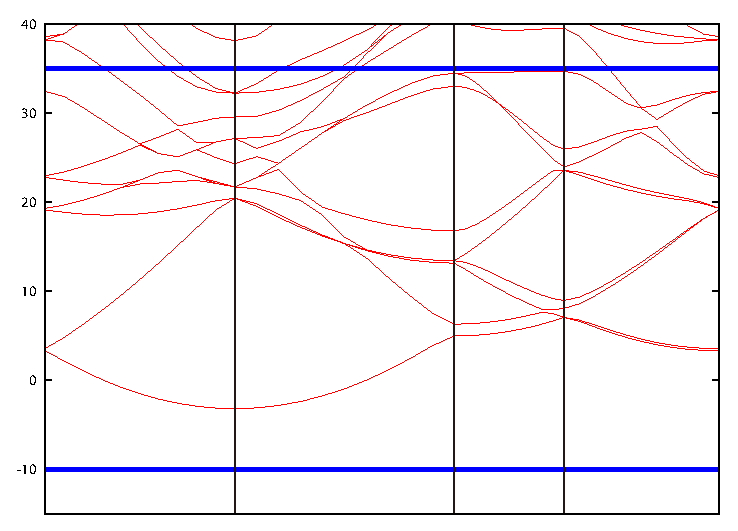
\includegraphics[width=8cm]{Energy-Window.Al.eps}
\caption{Band structure of Al. The lower limit of the energy window is $-10$ eV ({\tt Lower\_energy\_window=-10.0}) and the upper limit is +35 eV ({\tt Upper\_energy\_window=35.0}). From the bands in this window, nine Wannier functions ({\tt N\_wannier=9}) were created from nine initial Gaussian ({\tt N\_initial\_guess=9}).}
\label{EW}
\end{figure}

\verb+icell+ is a variable that specifies crystal lattice. \verb+icell=0+ is default which means an automatic search. \verb+EPS_SPILLAGE+, \verb+EPS_SPREAD+, \verb+DAMP+, \verb+MAX_STEP_LENGTH+ are parameters for convergence of the calculation. These are set to the default values.

\verb+set_inner_window+ is a parameter that specifies the inner energy window. \verb+Lower_inner_window+ and \verb+Upper_inner_window+ are variables that specify the inner energy window. When these parameters are specified, the Wannier functions are constructed so that the bands within the inner energy window coincides with the original bands. In this Al calculation, \verb+set_inner_window=F+, so the inner window is not set. Details of these parameters are described in La$_2$CuO$_4$ calculation (chapter \ref{La2CuO4}).

\verb+flg_initial_guess_direc+ is a variable specifying the coordinate system for displaying the Gaussian function. If you want to change to local coordinates instead of the Cartesian coordinates, you set \verb+flg_initial_guess_direc=1+. This flag is explained in TiO$_2$ calculation in the \ref{TiO2} chapter.

\verb+flg_BMAT+ is a variable related to the procedure for making the initial guess of the Wannier function. If \verb+flg_BMAT=1+, we linearly combine the Gaussians to make initial guess as follows:
\begin{eqnarray}
w_{j}^{in}({\bf r})=\sum_{i}B_{ij} g_i({\bf r}). \nonumber
\end{eqnarray} 
If \verb+flg_BMAT=0+, the linear combination is not performed, and hence the B matrix is an identity matrix. If \verb+flg_BMAT=1+ is set, the coefficient $B_{ij}$ of the linear combination is read following the information of the initial Gaussian. This will be explained in Si calculation in the \ref{Si} chapter. 

\tr{The variable {\tt electron\_number\_wannier\_space} specifies the number of electrons in the Wannier space. If this variable is set, the Fermi level is recalculated. The Fermi level is estimated so that the number of electrons ({\tt 3.0} in the present example) matches the numerical integral for the density of states until the Fermi level. The default is {\tt 0.0} and in this case the Fermi level obtained in the band calculation is employed.} 

\tr{Set {\tt flg\_global\_dos=1} if you want to calculate the density of states for the band energy obtained in the band calculation. The default is {\tt 0} and it is not calculated. The density of states in the Wannier space is always calculated.}

\tr{Set {\tt flg\_fermisurface=1} if you want to calculate the Fermi surface. The input of the Fermi-surface drawing software {\sc Fermisurfer} is output. The default is {\tt 0} and it is not calculated.} 
\vspace{-3mm}
\subsubsection{\&param\_interpolation}  
The namelist \verb+&param_interpolation+ contains input variables for drawing the Wannier-interpolation band. The interpolation-band calculation is always performed, so variables in this namelist are almost required parameters. An error occurs if you forget to specify the required parameters. Variable explanations are indicated in the right of \verb+!+. 
\vspace{5mm}\hrule
\begin{verbatim}
&param_interpolation   
N_sym_points=5,   !n: Total number of symmetric k points in calculation lines
Ndiv=40/          !o: Number of divisions between symmetric k points
0.500 0.500 0.500 !n: Symmetric k point; SK_sym_pts(1:3,1); L
0.000 0.000 0.000 !n: Symmetric k point; SK_sym_pts(1:3,2); G
0.500 0.000 0.500 !n: Symmetric k point; SK_sym_pts(1:3,3); X
0.500 0.250 0.750 !n: Symmetric k point; SK_sym_pts(1:3,4); W
0.500 0.500 0.500 !n: Symmetric k point; SK_sym_pts(1:3,5); L 
\end{verbatim}
\hrule\vspace{3mm}
In this namelist, you specify the number of symmetric $k$ points in the Brillouin zone, \verb+N_sym_points+. \verb+Ndiv+ is the number of divisions between two symmetric $k$ points and is an optional parameter. The default value is \verb+40+. Below this namelist, give the coordinates of the symmetric $k$ point (in reciprocal lattice coordinates). It is desirable to compare the original bands obtained by the band calculation with the Wannier-interpolation bands, and to check whether the latter is well reproduced the former.

\subsubsection{\&param\_visualization} 

The namelist \verb+&param_visualization+ contains input variables for drawing the realspace Wannier function. When calculation was completed, the realspace Wannier function data for drawing in visualization software {\sc VESTA} (http://jp-minerals.org/vesta/jp/) is generated.
\vspace{5mm}\hrule
\begin{verbatim}
&param_visualization   
flg_vis_wannier=1,!o: Calculate realspace Wannier function (do not: 0, do 1)
N_write_wannier=9,!o: Total number of realspace Wannier functions to be calculated
ix_vis_min=-1,    !o: Draw range of Wannier function (starting lattice in a1 direction)
ix_vis_max= 1,    !o: Draw range of Wannier function (end lattice in a1 direction)
iy_vis_min=-1,    !o: Draw range of Wannier function (starting lattice in a2 direction)
iy_vis_max= 1,    !o: Draw range of Wannier function (end lattice in a2 direction)
iz_vis_min=-1,    !o: Draw range of Wannier function (starting lattice in a3 direction)
iz_vis_max= 1,    !o: Draw range of Wannier function (end lattice in a3 direction)
\end{verbatim}
\hrule\vspace{5mm}
If you want to calculate the realspace Wannier function, you set \verb+flg_vis_wannier=1+. The default is \verb+0+, which does not perform calculation. \verb+N_write_wannier+ is the number of the realspace Wannier functions you want to calculate. By default, this variable is set to \verb+N_wannier+. You can specify fewer than \verb+N_wannier+. In this case, the program calculates \verb+N_write_wannier+ species of the Wannier functions (see chapter \ref{select-wannier}).

\subsection{\label{job-wannier}Execute job}
The job is executed as follows. The commands in the sh system are as follows.
\vspace{3mm}\hrule
\begin{verbatim}
export OMP_NUM_THREADS=16
export MKL_NUM_THREADS=16
./calc_wannier < input.in > LOG.wannier  
\end{verbatim}
\hrule\vspace{3mm}
\verb+calc_wannier+ is an executable file for calculating the Wannier function. Jobs are executed with \verb+input.in+ placed in the current directory and band-calculation files placed in \verb+./dir-wfn+. This job is \verb+openmp+ job (using 16 threads). The standard output of the calculation is output to \verb+LOG.wannier+.
\vspace{-3mm}
\subsection{\label{result-wannier}Calculation results}
When the job is executed, the directory \verb+dir-wan+ is created under the calculation directory. The calculation result is output in this directory. The output file is as follows.
\vspace{3mm}\hrule
\begin{enumerate}
\item \verb+./dir-wan/dat.h_mat_r+ (Realspace transfer matrix)
\item \verb+./dir-wan/dat.iband+ (Wannier-interpolation band)
\item \verb+./dir-wan/dat.umat+ (Unitary matrix)
\item \verb+./dir-wan/dat.wan+ (Expansion coefficients of Wannier function)
\item \verb+./dir-wan/dat.wan-center+ (Position of center of Wannier function)
\item \verb+./dir-wan/dat.ns-nb+ (Band information considered in Wannier-function calculation)
\item \tr{{\tt ./dir-wan/dat.wan-realspace-001.grd} $\sim$ {\tt dat.wan-realspace-009.grd}} (Realspace Wannier function)
\item \tr{{\tt ./dir-wan/dat.supercell-002x002x002-Al.cif} (Crystal structure)}
\item \verb+./dir-wan/dat.frmsf+ (Fermi surface data)
\item \tr{{\tt ./dir-wan/dat.dos.global-total} (Density of state for band energies)}
\item \tr{{\tt ./dir-wan/dat.dos.wan-total} (Density of states in Wannier space)} 
\item \tr{{\tt ./dir-wan/dat.dos.wan-001} $\sim$ {\tt dat.dos.wan-009} (Partial density of states)}  
\end{enumerate}
\hrule \vspace{3mm}

\verb+dat.h_mat_r+ contains data for the realspace transfer matrix: the Kohn-Sham Hamiltonian matrix elements with the Wannier function $\langle w_{i{\bf 0}}|h_{KS}|w_{j{\bf R}}\rangle$. The range of the lattice ${\bf R}$ is \verb+-Na1:Na1+ along the $a_1$ direction, \verb+-Na2:Na2+ along the direction of $a_2$, \verb+-Na3:Na3+ along the $a_3$ direction (The values of \verb+Na1+, \verb+Na2+, \verb+Na3+ are automatically set from the sample-$k$ point number).

In this program, the $i$ th Wannier function of the lattice {\bf R} is defined as follows:
\begin{eqnarray}
w_{i{\bf R}}({\bf r})=\frac{1}{\sqrt{N}}\sum_{{\bf k}}^{N}e^{-i{\bf kR}} \sum_{\alpha=N_s({\bf k})}^{N_b({\bf k})} U_{\alpha i}^{{\bf k}} \psi_{\alpha{\bf k}}({\bf r}), \label{wir}
\end{eqnarray} 
where $N$ is the total number of Monkhorst-Pack $k$ mesh. $N_s({\bf k})$ is the starting point number of the bands used to make the Wannier function, and $N_b({\bf k}) $ is the total number of those bands, which are automatically calculated from the energy-window information. $N_s({\bf k}), N_b({\bf k})$ are stored in \verb+dat.ns-nb+, and the transformation matrix \{$U_{\alpha i}^{{\bf k}}$\} is contained in \verb+dat.umat+. Note that these quantities depend on the $k$ point. $\psi_{\alpha {\bf k}}({\bf r})$ is the Bloch wave function and is defined as follows: 
\begin{eqnarray}
\psi_{\alpha{\bf k}}({\bf r})=\frac{1}{\sqrt{N}} \sum_{{\bf G}} c_{{\bf k+G},\alpha} \frac{1}{\sqrt{\Omega}} e^{i({\bf k+G})\cdot{\bf r}},  \label{pak} 
\end{eqnarray} 
where $\Omega$ is the volume of the calculation cell. Both the Wannier function $w_{i {\bf R}}({\bf r})$ and the Bloch function $\psi_{\alpha{\bf k}}({\bf r})$ are normalized in the crystal volume. When one inserts Eq.~(\ref{pak}) into the Eq.~(\ref{wir}), the Wannier function at the home cell ({\bf R=0}) is written as
\begin{eqnarray}
w_{i{\bf 0}}({\bf r})
=\frac{1}{N}
\sum_{{\bf k}}^{N}
\sum_{{\bf G}} 
\tilde{c}_{{\bf k+G},i}
\frac{1}{\sqrt{\Omega}}
e^{i({\bf k+G})\cdot{\bf r}} 
\end{eqnarray}
with 
\begin{eqnarray} 
\tilde{c}_{{\bf k+G},i}=\sum_{\alpha=N_s({\bf k})}^{N_b({\bf k})} U_{\alpha i}^{{\bf k}} c_{{\bf k+G},\alpha} \label{cikg}.  
\end{eqnarray}
Here, \{$w_{i {\bf 0}}({\bf r})$\} are stored in \verb+dat.wan-realspace-@@@.grd+ (\verb+@@@+ is the number of the output Wannier function, $i$). Also, \{$\tilde{c}_{i \bf k+G}$\} are stored in \verb+dat.wan+.

\tr{{\tt dat.iband} is the Wannier-interpolation band and, in {\tt gnuplot}, is plotted as follows [Fig.~\ref{iband}(a)]. The density of states ({\tt dat.dos.global-total}) and the Wannier density of states ({\tt dat.dos.wan-total}) are also plotted with {\tt gnuplot}. These are shown in Fig.~\ref{iband}(b). The third column of {\tt dat.dos.global-total} and/or {\tt dat.dos.wan-total} contains data of the step function $H(E_F-\omega)$. The unit of the density of states is {\tt states/eV}, which is defined as the total number of states including the spin degeneracy 2.}
\vspace{3mm}\hrule
\begin{verbatim}
gnuplot> plot 'dir-wan/dat.iband' w line 
gnuplot> plot 'dir-wan/dat.dos.global-total', 'dir-wan/dat.dos.global-total' u 1:3, 
              'dir-wan/dat.dos.wan-total'
\end{verbatim}
\hrule\vspace{3mm}
\begin{figure}[H] 
\centering
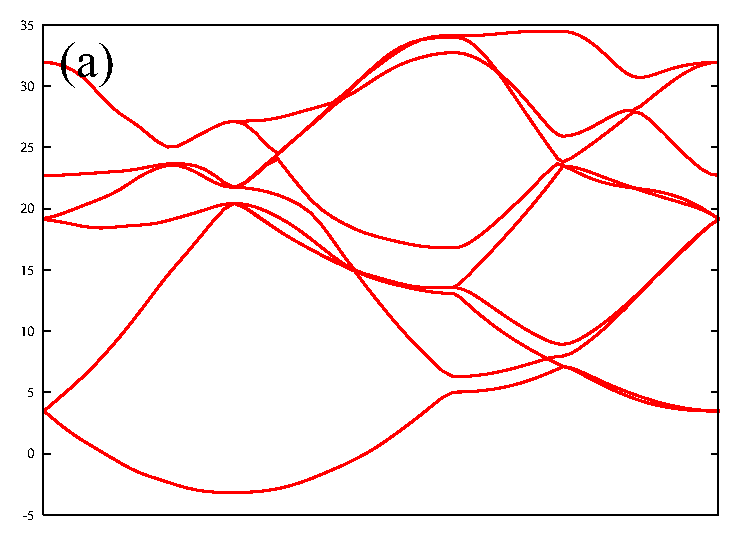
\includegraphics[width=6cm]{dat.iband-Al.eps}
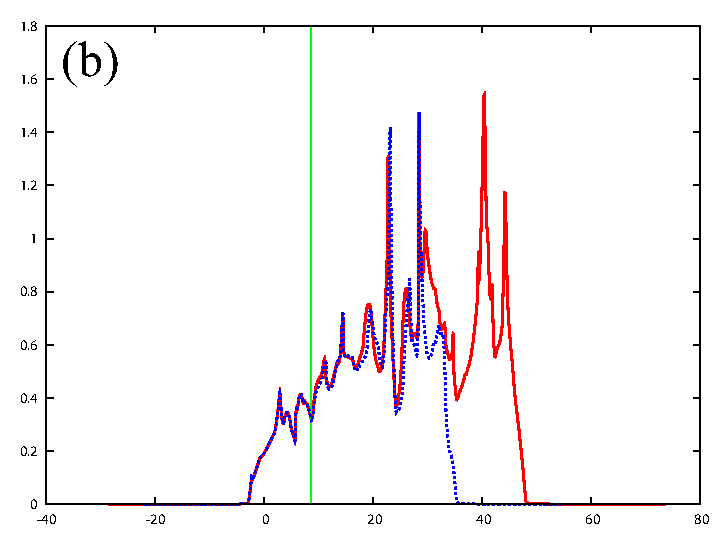
\includegraphics[width=6cm]{dat.dos-Al.eps}
\caption{Calculated Wannier interpolation band. Unit of vertical axis is {\tt eV}. \tr{(b) Calculated density of states (red: global, green: step function at Fermi level, blue: the Wannier density of states). The unit of the horizontal and vertical axes are {\tt eV} and {\tt states/eV}, respectively.}} 
\label{iband}
\end{figure}

\tr{The plot for the partial density of states is also shown in Fig.~\ref{pdos} with {\tt gnuplot}. Only the contributions of the $s$ and $d_{x^2-y^2}$ orbitals are shown.}
\vspace{3mm}\hrule
\begin{verbatim}
gnuplot> plot 'dir-wan/dat.dos.wan-total', 'dir-wan/dat.dos.wan-001' u 1:3, 
              'dir-wan/dat.dos.wan-009' 
\end{verbatim}
\hrule\vspace{3mm}
\begin{figure}[H] 
\centering
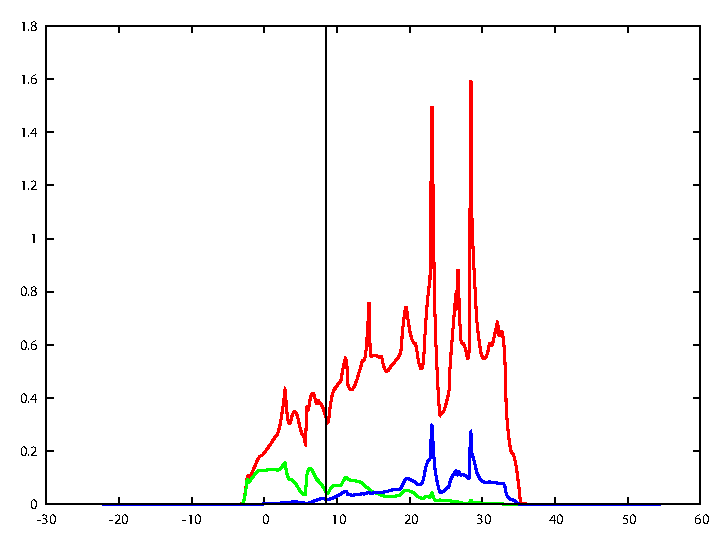
\includegraphics[width=7cm]{dat.pdos-Al.eps}
\caption{\tr{Partial density of states: Red is the Wannier density of state, green is the contribution from the $s$ orbital, and blue is the contribution from the $d_{x^2-y^2}$ orbital. The unit of the horizontal and vertical axes are {\tt eV} and {\tt states/eV}, respectively.}}  
\label{pdos}
\end{figure}

\tr{Figure~\ref{vesta} displays the atomic structure and the realspace Wannier function with {\sc VESTA}: {\tt dat.supercell-002x002x002-Al.cif} is a structure file whose size matches the display range of the Wannier function. In this case, the size is $2\times2\times2$. {\tt dat.wan-realspace-}{\it number}{\tt .grd} is the realspace Wannier function data ({\it number} is the number of Wannier function). This figure can be created simply by reading {\tt dat.supercell-002x002x002-Al.cif} and {\tt dat.wan-realspace-}{\it number}{\tt .grd} into {\sc VESTA}.}  
\begin{figure}[H] 
\centering
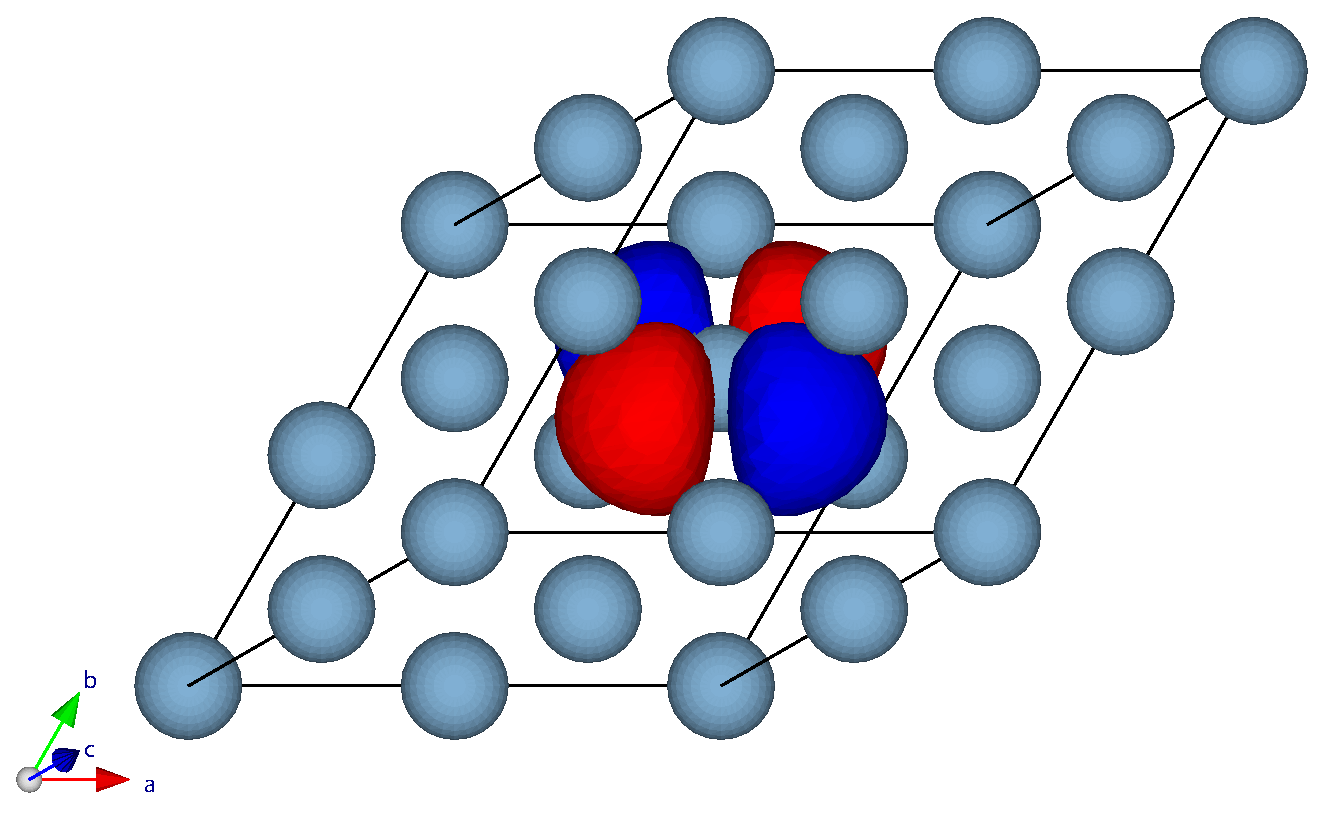
\includegraphics[width=8cm]{dat.wan-realspace-Al.eps}
\caption{Realspace Wannier function. The 9th Wannier function ({\tt dat.wan-realspace-009.grd}) is drawn, which is the $d_{x^2-y^2}$ orbital. \tr{Atomic structure data {\tt dat.supercell-002x002x002-Al.cif} and $d_{x^2-y^2}$ Wannier function data ({\tt dat.wan-realspace-009.grd}) are superposed. We use the visualization software {\sc VESTA} ({\tt https://jp-minerals.org/vesta/jp/}).}} 
\label{vesta}
\end{figure}

\tr{Figure~\ref{frmsf-in-wannier-code} displays the calculated Fermi surface with the Fermi surface drawing software {\sc FermiSurfer}.} \verb+dat.frmsf+ is the Fermi surface data and is output in the reading form of {\sc FermiSurfer}. If {\sc FermiSurfer} is installed, you can make this plot simply by clicking \verb+dat.frmsf+.
\begin{figure}[H] 
\centering
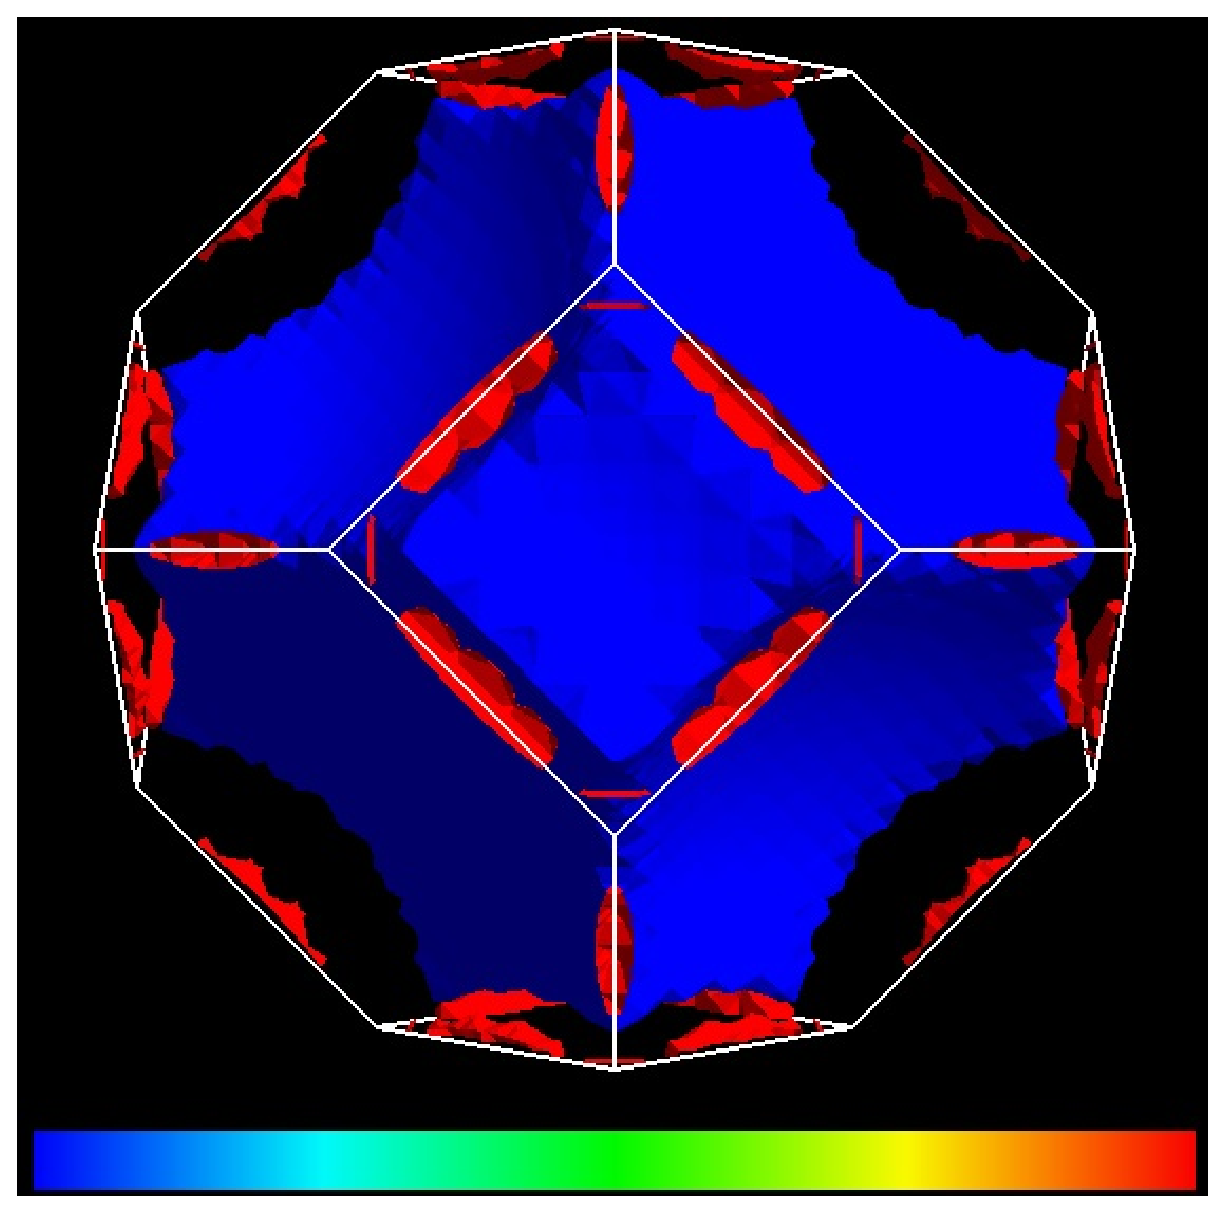
\includegraphics[width=6cm]{Al-21x21x21-frmsf.eps}
\caption{\tr{The Fermi surface drawn by the Fermi surface drawing software {\sc FermiSurfer} ({\tt https://ja.osdn.net/projects/fermisurfer/}). In this calculation, we used dense $k$-point sampling of $21\times21\times21$.}} 
\label{frmsf-in-wannier-code}
\end{figure}

\clearpage

\section{chiqw}

\subsection{\label{input-chiqw}Input file (\&param\_chiqw)}
Below is the input file \verb+input.in+ for the dielectric function calculation of Al. \verb+&param_chiqw+ is the name of the namelist, and variables are listed below this line. \tr{A brief description of variables is given in the right of {\tt !}. In {\tt \&param\_chiqw}, all variables are optional parameters, and the user may omit the input. Default values are presented in this list.} 
\vspace{5mm}\hrule
\begin{verbatim}
&param_chiqw 
Ecut_for_eps=3.6d0,           !o: Cutoff of polarization function (Ry)
Num_freq_grid=70,             !o: Total number of calculation frequencies
N_CALC_BAND=50,               !o: Total number of bands considered in polarization calc.
MPI_num_proc_per_qcomm=6,     !o: Number of MPI process per community
MPI_num_qcomm=1,              !o: Number of communities
MPI_io_rank=0,                !o: MPI number to be outputted to standard output
shift_ef=0.0d0,               !o: Artificial shift of Fermi level (eV)
Max_excitation_energy=200.0d0,!o: Maximum excitation energy to be considered in calc. (eV)
Green_func_delt=0.1d0,        !o: Smearing value in tetrahedron calculation (eV)
ttrhdrn_dmna=1.0d-3,          !o: Degeneracy judge parameter in tetrahedron calc. (eV)
ttrhdrn_dmnr=1.0d-3,          !o: Degeneracy judge parameter in tetrahedron calc. (eV)
flg_cRPA=0,                   !o: constrained RPA option (0: RPA, 1: cRPA)
flg_calc_type=0               !o: 0: all-q-calc, 1: gamma-only, 2: bulk job
\end{verbatim}
\hrule\vspace{5mm}

\verb+Ecut_for_eps+ is the cutoff energy of the polarization function (unit: Ry). By default, it is set to 1/10 of the cutoff energy of the wave function used in the band calculation (in the Al case, since the wave function cutoff is 36 Ry, the polarization function cutoff is set to 3.6 Ry). \verb+Num_freq_grid+ is the total number of calculation frequencies of the polarization function. By default, a log grid of 70 points is generated. \verb+N_CALC_BAND+ is the number of bands considered in the polarization calculation. By default, the number of bands calculated in the band calculation is set. From this number of bands, the maximum excitation energy $E_{max}$ is determined. \tr{The calculated frequency is taken up to $3E_{max}$ by considering the Lorentz tail of the polarization function.}

\verb+MPI_num_proc_per_qcomm+, \verb+MPI_num_qcomm+, \verb+MPI_io_rank+ are parameters for MPI calculation. In the case of the above setting value, 6 MPI calculation is assumed, and the output is in charge of the master MPI. 
\tr{Parallel computation for $q$ points can be performed by setting the variable {\tt MPI\_num\_qcomm}, where ${\bf q}$ specifies the irreducible wavevector for the polarization function. This is discussed in more detail in Chapter~\ref{qcom}.} 

\verb+Green_func_delt+, \verb+ttrhdrn_dmna+, \verb+ttrhdrn_dmnr+ are parameters for tetrahedron calculation. All default values are prepared. \tr{{\tt shift\_ef} is used for artificially shift of the Fermi level (unit is eV).} \verb+Max_excitation_energy+ is set when you want to limit excitation energy (unit is eV).

\verb+flg_cRPA+ is a variable that specifies whether or not constrained RPA calculation is performed. By default, normal RPA calculation is performed, so \verb+flg_cRPA=0+. When performing constrained RPA calculation (\verb+flg_cRPA=1+), there are two strategies. One is to specify the exclusion of the polarization by the Wannier functions, and the other is to specify the exclusion of the polarization by specifying the energy window. The default is the former (if you want to use the latter option please contact me). {\tt In the case of the former, the {\tt wannier} calculation (Chapter~\ref{wannier}) must be executed before the {\tt chiqw} calculation.} The constrained RPA calculation will be described in detail in the subsequent La$_2$CuO$_4$ calculation (Chapter~\ref{La2CuO4}).

An option to specify the calculation $q$ point is also provided (\verb+flg_calc_type=2+). Details are described in Chapter~\ref{bulkjob}.

%Band calculation data for the \verb+chiqw+ calculation must be $k$ point data of Monkhorst-Pack mesh. The band calculation data for the \verb+chiqw+ calculation must be data calculated at the $k$ point of the Monkhorst-Pack mesh. The data \verb+dat.sample-k+, \verb+dat.nkm+, \verb+dat.eigenvalue+, \verb+dat.kg+, \verb+dat.wfn+ obtained for irreducible $k$ points are converted to all $k$-point data on the Monkhorst-Pack mesh by using symmetry information of \verb+dat.symmetry+.

\subsection{\label{job-chiqw}Execute job}
The job is executed as follows. Specifications in sh system are as follows.
\vspace{3mm}\hrule
\begin{verbatim}
export OMP_NUM_THREADS=16
export MKL_NUM_THREADS=16
mpirun -np 6 ./calc_chiqw < input.in > LOG.chiqw  
\end{verbatim}
\hrule\vspace{3mm}

\verb+calc_chiqw+ is an executable file for dielectric function calculation. \verb+calc_chiqw+ is created by compiling in the directory \verb+RESPACK/src/chiqw+ (see the \ref{compile} section). The job is executed with input file \verb+input.in+ and files in the directory \verb+./dir-wfn+. \tr{This job is a hybrid parallel job [total MPI processes are 6 ({\tt -np 6})  and each MPI process consists of 16 threads]. If you omit {\tt MPI\_num\_proc\_per\_qcomm} and {\tt MPI\_num\_qcomm}, {\tt MPI\_num\_proc\_per\_qcomm=6} and {\tt MPI\_num\_qcomm=1} are automatically set. {\tt input.in} is read as standard input. Standard output of calculation  is output to {\tt LOG.chiqw} (standard output is in charge by MPI master by default).}

\subsection{\label{result-chiqw}Calculation results}
When the job is executed, a directory \verb+dir-eqs+ is created under the calculation directory. 
\tr{In this directory, frequency-grid information ({\tt dat.wgrid}), polarization-function-cutoff information ({\tt dat.chi\_cutoff}), electron-energy-loss spectrum ({\tt dat.eels-x, -y, -z}), optical-absorption spectrum ({\tt dat.optical\_conductivity-x, -y, - z}), reflectivity ({\tt dat.reflectivity-x, -y, -z}) are output. Here, {\tt -x, -y, -z} attached to the spectrum represents a Cartesian coordinates.}
 \tr{Furthermore, the directory {\tt qxxx} attached with the $q$ point number ({\tt xxx}) is generated under the {\tt dir-eqs} directory. Calculation results for each $q$ point are output in this directory. Note that the number of $q$ points (i.e., the number of the {\tt qxxx} directories) is the number of irreducible $q$ points (16 in the Al calculation). For the files in each {\tt qxxx} directory, for example, in the case of the 16th $q$ point, the following output files are generated in the {\tt q016} directory.} 
\vspace{5mm}\hrule
\begin{enumerate}
\item \verb+./dir-eps/dat.wgrid+ (Frequency grid)
\item \tr{{\tt ./dir-eps/dat.chi\_cutoff} (Polarization cutoff)}
\item \tr{{\tt ./dir-eps/dat.ttrhdrn} (Tetrahedron parameters)} 
\item \tr{{\tt ./dir-eps/dat.eels-x (-y,-z)} (Electron-energy-loss spectrum)}
\item \tr{{\tt ./dir-eps/dat.optical\_conductivity-x (-y,-z)} (Optical-absorption spectrum)}
\item \tr{{\tt ./dir-eps/dat.reflectivity-x (-y,-z)} (Reflectance spectrum)} 
\item \verb+./dir-eps/q016/dat.log.400+ (Calculation end flag)
\item \verb+./dir-eps/q016/dat.epsqw.600+ (Inverse dielectric function data)
\item \verb+./dir-eps/q016/dat.epsqw.600001-dat.epsqw.600070+ (Diagonal terms of inverse dielectric matrix for each frequency)
\end{enumerate}
\hrule\vspace{5mm}

\verb+dat.log.400+ is the calculation end flag. Inverse dielectric matrix \{$\epsilon_{{\bf GG'}}^{-1}({\bf q},\omega)$\} is accommodated in \verb+dat.epsqw.600+ in the binary format. \tr{For the files of 600000 series ({\tt dat.epsqw.600000}$\sim${\tt dat.epsqw.600070}), we store the diagonal term data of the inverse dielectric matrix for each frequency grid.} The first column is $|{\bf q+G}|$ (unit is Bohr$^{- 1}$), the second column is $\epsilon_{{\bf GG}}^{-1}{\bf q}, \omega_i)$, and the third column is the imaginary part. In the case of this job (\verb+Num_freq_grid=70+), it is generated from \verb+dat.epsqw.600001+ to \verb+dat.epsqw.600070+. \tr{For example, {\tt dat.epsqw.600001}  contains the dielectric matrix at the first frequency $\omega_1$. Also, {\tt dat.epsqw.600070} contains the diagonal term of the dielectric matrix $\epsilon_{{\bf GG}}^{-1}({\bf q}, \omega_{70})$. On the plot of $\epsilon_{{\bf GG}}^{-1}({\bf q},\omega)$, perform the following procedure. Here we plot the result of $\omega^{-1}=0$. The result is shown in Fig.~\ref{epsqw}.}  
\vspace{3mm}\hrule
\begin{verbatim}
cat dir-eps/q0*/dat.epsqw.600001 > epsq0
gnuplot
gnuplot> plot 'epsq0' u 1:2,'epsq0' u 1:3  
\end{verbatim}
\hrule\vspace{3mm}
\begin{figure}[H] 
\centering
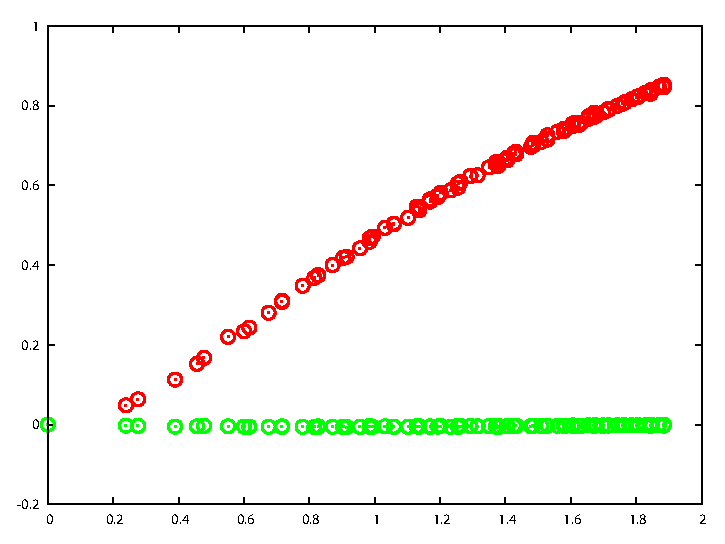
\includegraphics[width=8cm]{epsq0-Al.eps}
\caption{Diagonal terms of of the inverse dielectric matrix for the all $q$ points $\epsilon_{{\bf GG}}^{-1}({\bf q}, \omega_1)$ (Red is the real part, green is the imaginary part). The horizontal axis is $|{\bf q+G}|$ (Bohr $^{-1}$). In this result, the result at $\omega_1=0$ is plotted.}
\label{epsqw}
\end{figure}

\tr{The output of the electronic energy loss spectrum, the optical absorption spectrum, and the reflectance is plotted as follows with {\tt gnuplot}:} 
\vspace{3mm}\hrule
\begin{verbatim} 
gnuplot 
gnuplot> plot `dat.eels-x', `dat.eels-x' u 1:3 
gnuplot> plot `dat.optical_conductivity-x', `dat.optical_conductivity-x' u 1:3 
gnuplot> plot `dat.reflectivity-x' 
\end{verbatim}
\hrule\vspace{3mm}
\begin{figure}[H] 
\centering
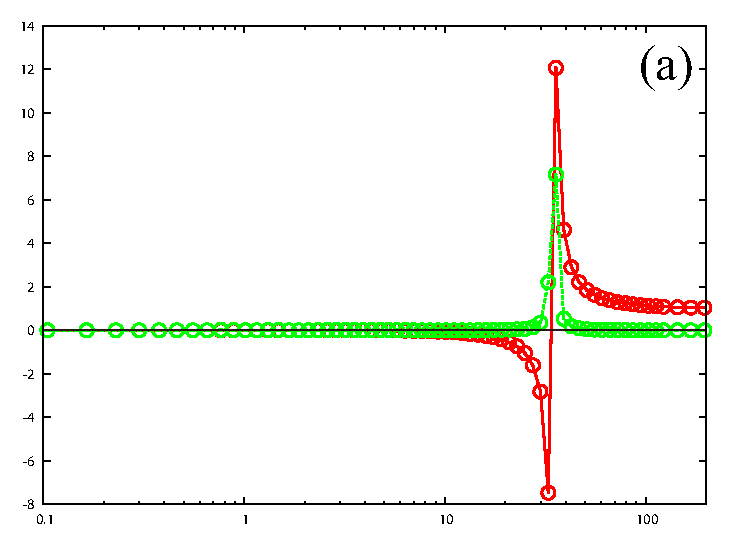
\includegraphics[width=8cm]{eels-Al.eps}
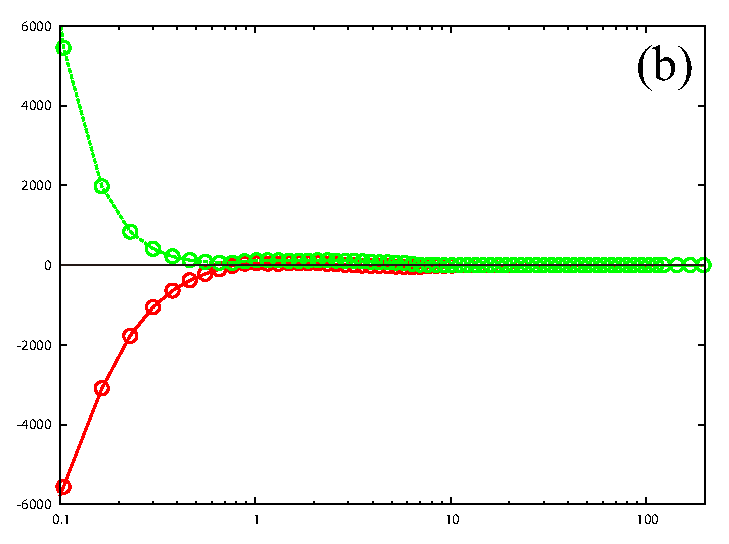
\includegraphics[width=8cm]{optical_conductivity-Al.eps}
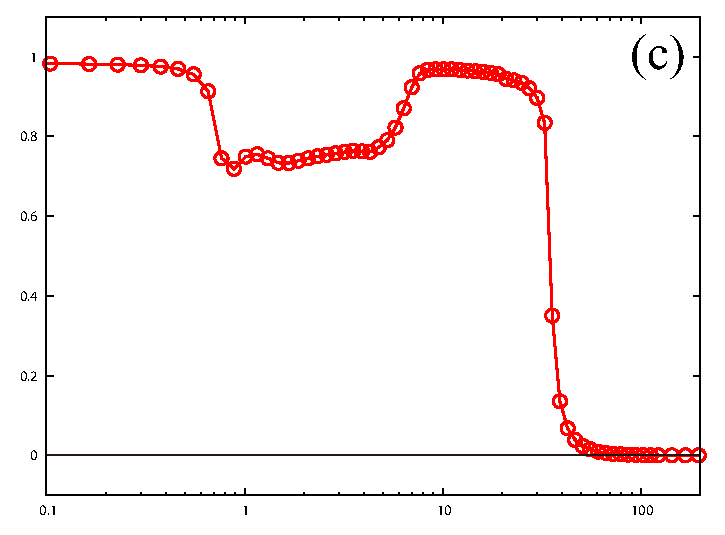
\includegraphics[width=8cm]{reflectivity-Al.eps}
\caption{\tr{(a) Calculation result for the electronic energy loss spectrum. Red is the real part, green is the imaginary part. The horizontal axis is $\omega$ (Hartree). A large peak (green) appears at about 30 eV, which is the intensity due to Al plasmon absorption. (b) Optical absorption spectrum. Red is the real part, green is the imaginary part. (c) Reflectance spectrum.}} 
\label{eels}
\end{figure}

\clearpage 

\section{calc\_w3d and calc\_j3d}
\tr{Evaluations of direct and exchange integrals are executed in separate executable files (direct-integral calculation is performed with {\tt calc\_w3d}, exchange-integral calculation is {\tt calc\_j3d}), which can be performed with common inputs. Note that the integral evaluation must be done after the {\tt wannier} and {\tt chiqw} calculation.} 

\subsection{\label{input-calc-int}Input file (\&param\_calc\_int)}
Below is the input file \verb+input.in+ for the interaction-integral evaluation (\verb+calc_w3d+, \verb+calc_j3d+). Default values are prepared for all variables in the namelist \verb+&param_calc_int+.
\vspace{3mm}\hrule
\begin{verbatim}
&param_calc_int 
calc_ifreq=1, !o: Frequency to be calculated
ix_int_min=0, !o: Calc. range of exchange (start lattice in a1 direc.) (calc_j3d only)
ix_int_max=0, !o: Calc. range of exchange (end lattice in a1 direc.) (calc_j3d only)
iy_int_min=0, !o: Calc. range of exchange (start lattice in a2 direc.) (calc_j3d only)
iy_int_max=0, !o: Calc. range of exchange (end lattice in a2 direc.) (calc_j3d only)
iz_int_min=0, !o: Calc. range of exchange (start lattice in a3 direc.) (calc_j3d only)
iz_int_max=0/ !o: Calc. range of exchange (end lattice in a3 direc.) (calc_j3d only)
\end{verbatim}
\hrule\vspace{3mm}
\tr{The important point in performing the integral calculation is to calculate the inverse dielectric matrix of all irreducible $q$ points before this calculation.} This is because it is impossible to generate all the data on the Monkhorst-Pack mesh if the data at the irreducible $q$ point is insufficient. RESPACK checks the presence/absence of end flag of the dielectric calculation \verb+dat.log.400+ in the directories  \verb+./dir-eps/qxxx+, and stops calculation when there is not.

\subsection{\label{job-calc-int}Execute job}
The job is executed as follows. Specifications in sh system are as follows.
\vspace{3mm}\hrule
\begin{verbatim}
export OMP_NUM_THREADS=16
export MKL_NUM_THREADS=16
./calc_w3d (or ./calc_j3d) < input.in > LOG.W3d (or LOG.J3d)  
\end{verbatim}
\hrule\vspace{3mm}
\verb+calc_w3d+ or \verb+calc_j3d+ are executable files for interaction-integral calculation. The job is executed with the input file \verb+input.in+ placed in the current directory and the files placed in the directories \verb+./dir-wfn+, \verb+./dir-eps+, \verb+./dir-wan+. This job is \verb+openmp+ job (using 16 threads). The standard output of \verb+calc_w3d+ is output to \verb+LOG.W3d+, and the standard output of \verb+calc_j3d+ is output to \verb+LOG.J3d+.

\subsection{\label{result-calc-int}Calculation results}
When the job is executed, \verb+dir-intW+ and \verb+dir-intJ+ are created under the calculation directory, and the calculation result is output in these directories; the results of \verb+calc_w3d+ is contained in \verb+dir-intW+, and the result of \verb+calc-j3d+ is contained in \verb+dir-intJ+. The output files are as follows.
\vspace{3mm}\hrule
\begin{enumerate}
\item \verb+./dir-intW/dat.Wmat+ [Screened direct integral, Eq (5)]
\item \verb+./dir-intW/dat.Vmat+ [Bare direct integral, Eq (7)] 
\item \verb+./dir-intW/dat.VvsR.001 - dat.VvsR.009+ ($V(r)$) 
\item \verb+./dir-intW/dat.WvsR.001 - dat.WvsR.009+ ($W(r)$)
\item \verb+./dir-intW/dat.UvsE.001-001 - dat.UvsE.009-009+ ($U(\omega)$)
\item \verb+./dir-intJ/dat.Jmat+ [Screened exchange integral, Eq (6)] 
\item \verb+./dir-intJ/dat.Xmat+ [Bare exchange integral, Eq (8)]
\item \verb+./dir-intJ/dat.JvsE.001-001 - dat.JvsE.009-009+ ($J(\omega)$)
\end{enumerate}
\hrule\vspace{3mm}
\tr{The screened direct and exchange integrals are defined as follows:}  
\begin{eqnarray}
W_{ij}({\bf R},\omega)&=&\int_V d{\bf r} \int_V  d{\bf r'}
w_{i{\bf 0}}^*({\bf r}) 
w_{i{\bf 0}}({\bf r}) 
W({\bf r,r'},\omega) 
w_{j{\bf R}}^*({\bf r'}) 
w_{j{\bf R}}({\bf r'}), \label{Wij} \\
J_{ij}({\bf R},\omega)&=&\int_V  d{\bf r}\int_V d{\bf r'}
w_{i{\bf 0}}^*({\bf r}) 
w_{j{\bf R}}({\bf r}) 
W({\bf r,r'},\omega) 
w_{j{\bf R}}^*({\bf r'}) 
w_{i{\bf 0}}({\bf r'}). \label{Jij}
\end{eqnarray}
\tr{The integral is performed over the crystal volume $V$. These integrals are matrix element of the screened Coulomb interaction $W({\bf r,r'} \omega)$ between the $i$th Wannier function of the home cell ({\bf R=0}) and the $j$th Wannier function of the cell {\bf R}. In the case of a bare Coulomb interaction $v({\bf r,r'})=${\Large $\frac{1}{|{\bf r-r'}|}$} instead of $W({\bf r,r'}.\omega)$, the bare direct and exchange integrals are defines as follows:} 
\begin{eqnarray}
V_{ij}({\bf R})&=&\int_V d{\bf r} \int_V  d{\bf r'}
w_{i{\bf 0}}^*({\bf r}) 
w_{i{\bf 0}}({\bf r}) 
v({\bf r,r'}) 
w_{j{\bf R}}^*({\bf r'}) 
w_{j{\bf R}}({\bf r'}), \label{Vij} \\
X_{ij}({\bf R})&=&\int_V  d{\bf r}\int_V d{\bf r'}
w_{i{\bf 0}}^*({\bf r}) 
w_{j{\bf R}}({\bf r}) 
v({\bf r,r'}) 
w_{j{\bf R}}^*({\bf r'}) 
w_{i{\bf 0}}({\bf r'}). \label{Kij}
\end{eqnarray}
Calculated data of \verb+dat.Wmat+, \verb+dat.Jmat+, \verb+dat.Vmat+, \verb+dat.Xmat+ are output as a matrix of \tr{{\tt N\_wannier}$\times${\tt N\_wannier} of each cell {\bf R}. The direct integral is calculated for all {\bf R}, while the exchange integral is calculated only in the lattice {\tt ix\_intJ\_min}$\sim${\tt iz\_intJ\_max}, because they are heavy calculations.} 

\tr{{\tt dat.WvsR.}{\it number} contains the distance dependence of the static screened direct integral [$W_{ij}({\bf R},0)$] ({\it number} specifies the number of the Wannier function)}. The direct integrals between the $i$the Wannier function of the home cell {\bf R=0} and all the Wannier functions at {\bf R} are calculated. By default, $\omega=0$ is calculated (\verb+calc_ifreq=1+), but by changing this variable you can calculate finite $\omega$ results. In the Al calculation, \verb+N_wannier=9+, so nine files are output. To see the screened effect, you might plot \tr{the bare interaction results {\tt dat.VvsR.}{\it number} together.} The output is as follows (Fig.~\ref{WvsR}):
\vspace{3mm}\hrule
\begin{verbatim}
gnuplot> plot 'dir-intW/dat.VvsR.001', 'dir-intW/dat.WvsR.001'  
\end{verbatim}
\hrule\vspace{3mm}
\begin{figure}[H] 
\centering
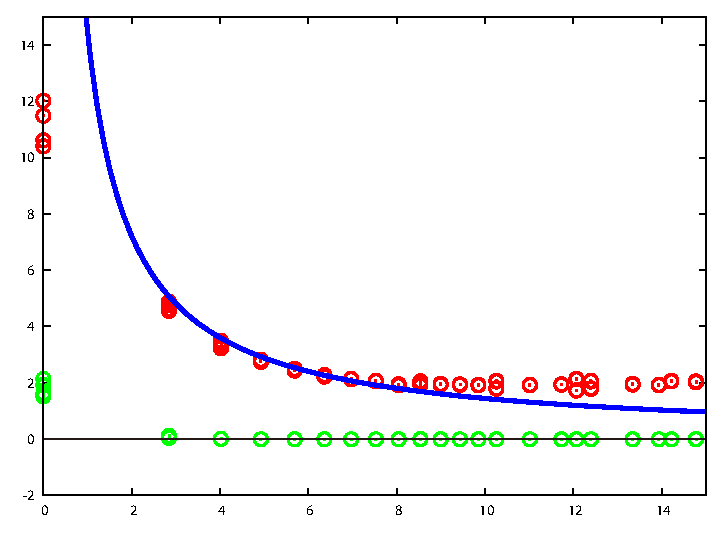
\includegraphics[width=8cm]{WvsR-Al.eps}
\caption{\tr{Distance dependence of bare direct integral (red) and static screened direct integral (green). The horizontal axis is the distance (unit: \AA) between the Wannier functions $w_{i{\bf 0}}$ and $w_{j{\bf R}}$, and the unit of the vertical axis is {\tt eV}. This result is for $i$={\tt 001}. The bare direct integrals are attenuated with ${\Huge \frac{1}{R}}$ (blue), while the static screened direct integrals have values only onsite due to metallic screening.}}
\label{WvsR}
\end{figure}

\tr{The frequency dependence of onsite screened direct integrals $W_{ii}({\bf 0},\omega)$ ({\tt dat.UvsE.}{\it number}{\tt -}{\it number}) is plotted as follows (Fig.~\ref{UvsE}). This output is $W_{11}({\bf 0},\omega)$, but, in the program, all $W_{ij}({\bf 0},\omega)$ are calculated for all pairs of the Wannier functions $i$ and $j$.}  
\vspace{3mm}\hrule
\begin{verbatim}
gnuplot> plot 'dir-intW/dat.UvsE.001-001' u 1:3, 'dir-intW/dat.UvsE.001-001' u 1:4  
\end{verbatim}
\hrule\vspace{3mm}
\begin{figure}[H] 
\centering
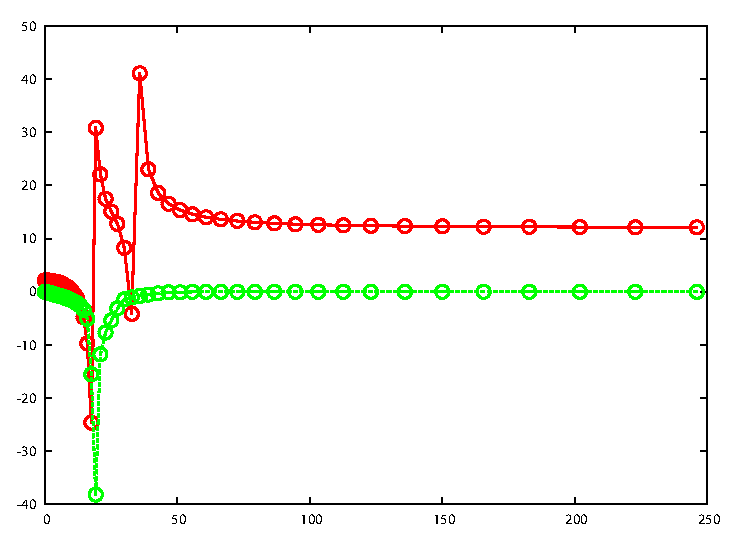
\includegraphics[width=8cm]{UvsE-Al.eps}
\caption{Frequency dependence of onsite screened direct integrals. Red is the real part, and green is the imaginary part. The horizontal axis shows the frequency $\omega$ ({\tt eV}), and the unit of the vertical axis is {\tt eV}. A pole due to the plasmon excitation can be seen around 20 eV.}
\label{UvsE}
\end{figure}

\tr{The frequency dependence of onsite screened exchange integrals [$J_ {ij}({\bf 0},\omega)$] is plotted as follows (Fig.~\ref{JvsE}). This output is $J_{12}({\bf 0},\omega)$, but, in the program, all $J_{ij}({\bf 0},\omega)$ are calculated for all pairs of the Wannier functions $i$ and $j$.}  
\vspace{5mm}\hrule
\begin{verbatim}
gnuplot> plot 'dir-intJ/dat.JvsE.001-002' u 1:3, 'dir-intJ/dat.JvsE.001-002' u 1:4  
\end{verbatim}
\hrule\vspace{5mm}
\begin{figure}[H] 
\centering
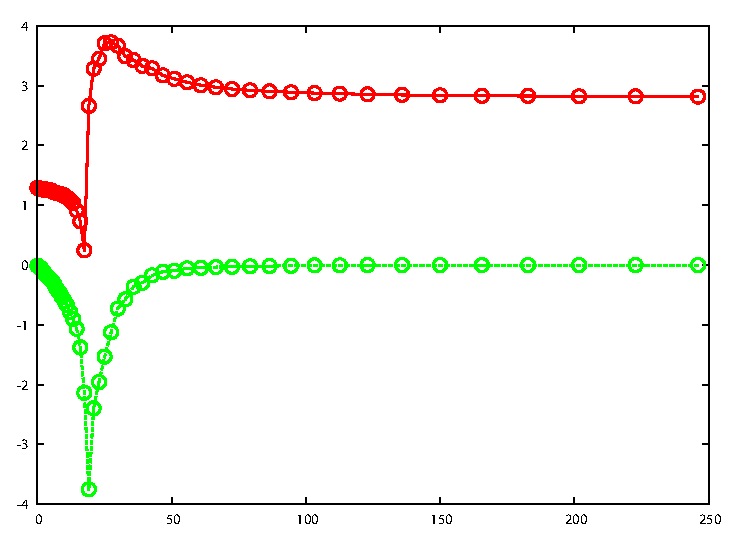
\includegraphics[width=8cm]{JvsE-Al.eps}
\caption{Frequency dependence of onsite screened exchange integrals. Red is the real part, and green is the imaginary part. The horizontal axis shows the frequency $\omega$ ({\tt eV}), and the unit of the vertical axis is {\tt eV}. We also see a pole around 20 eV, but the overall energy scale is about 1/10 of direct integral.}
\label{JvsE}
\end{figure}

\clearpage 

\section{\label{Al-summary}Summary: Al calculation input} 
\tr{We shows the final input of RESPACK calculation for Al, where all the optional variables are omitted. We can easily understand that necessary parameters are only for {\tt wannier} calculation, and other programs are default setting.} 
\vspace{3mm}\hrule
\begin{verbatim}
&param_wannier 
 N_wannier=9,                !n: Number of Wannier functions you want to calculate
 Lower_energy_window=-10.0d0,!n: Lower limit of energy window (eV)
 Upper_energy_window= 35.0d0,!n: Upper limit of energy window (eV)
 N_initial_guess=9/          !n: Number of initial Gaussian
 s   0.2d0 0.0d0 0.0d0 0.0d0 !n: Orbital type, Gaussian width, Gaussian position s@Al
 px  0.2d0 0.0d0 0.0d0 0.0d0 !n: px@Al
 py  0.2d0 0.0d0 0.0d0 0.0d0 !n: py@Al
 pz  0.2d0 0.0d0 0.0d0 0.0d0 !n: pz@Al
 dxy 0.2d0 0.0d0 0.0d0 0.0d0 !n: dxy@Al
 dyz 0.2d0 0.0d0 0.0d0 0.0d0 !n: dyz@Al
 dz2 0.2d0 0.0d0 0.0d0 0.0d0 !n: dz2@Al
 dzx 0.2d0 0.0d0 0.0d0 0.0d0 !n: dzx@Al
 dx2 0.2d0 0.0d0 0.0d0 0.0d0 !n: dx2-y2@Al
&param_interpolation   
 N_sym_points=5/   !n: Total number of symmetric k points in calculation lines
 0.500 0.500 0.500 !n: Symmetric k point; SK_sym_pts(1:3,1); L
 0.000 0.000 0.000 !n: Symmetric k point; SK_sym_pts(1:3,2); G
 0.500 0.000 0.500 !n: Symmetric k point; SK_sym_pts(1:3,3); X
 0.500 0.250 0.750 !n: Symmetric k point; SK_sym_pts(1:3,4); W
 0.500 0.500 0.500 !n: Symmetric k point; SK_sym_pts(1:3,5); L 
&param_visualization
 /  
&param_chiqw 
 /
&param_calc_int 
 /
\end{verbatim}
\hrule\vspace{3mm}

In this demonstration, the calculation condition is loosened to shorten the calculation time. For convergence, it is necessary to make strict conditions. The Wannier function mainly depends on the density of the $k$ points and the wave function cutoff. The dielectric function depends on the number of unoccupied bands and the dielectric function cutoff. For the Al calculation, it is better to take 10$\times$10$\times$10-$k$ points, wave function cutoff 64 Ry, dielectric function cutoff 10 Ry, and unoccupied band number 50. In the case of constrained RPA, it is generally better to include the unoccupied bands up to several tens of eV above the Fermi level.

\clearpage 

\section{\tr{Transfer analysis}}
\tr{When the RESPACK job ({\tt wannier, chiqw, calc\_w3d, calc\_j3d}) is completed, a directory {\tt ./dir-model} is created under the calculation directory, in which the following files are generated:}
\vspace{3mm}\hrule
\begin{enumerate}
\item \verb+./dir-model/zvo_hr.dat+ (transfer integrals)
\item \verb+./dir-model/zvo_dr.dat+ (density matrix)
\item \verb+./dir-model/zvo_ur.dat+ (direct Coulomb integrals)
\item \verb+./dir-model/zvo_jr.dat+ (exchange integrals)
\item \verb+./dir-model/zvo_geom.dat+ (Wannier centers: text format)
\item \verb+./dir-model/zvo_geom.xsf+ (Wannier centers: xsf format)
\item \verb+./dir-model/zvo_mkkpts.dat+ (k-grid information)
\item \verb+./dir-model/zvo_bandkpts.dat+ (k-grid information for band dispersion)
\item \verb+./dir-model/zvo_ef.dat+ (Fermi energy)
\end{enumerate}
\hrule\vspace{3mm}
\tr{These files are used for model-parameter analysis. On top of that, these files are inputs for model-solver software (mVMC and $\mathcal{H}\Phi$).  For the connection to mVMC and $\mathcal{H}\Phi$, see the site \texttt{https://issp-center-dev.github.io/mVMC/docs/index.html} for mVMC and \\   \texttt{http://issp-center-dev.github.io/HPhi/index.html} for $\mathcal{H}\Phi$.}

\tr{RESPACK provides a function to analyze transfer data. Using {\sc Python} script {\tt tr.py} and the executable files {\tt calc\_tr} from {\sc FORTRAN} code. User can execute the transfer analysis by coping these files to the calculation directory. Preparation for the calculations is as follows:} 
\vspace{3mm}\hrule\vspace{3mm}
\tr{\texttt{cd RESPACK/src/transfer\_analysis}}

\tr{\texttt{make}} 

\tr{\texttt{cp calc\_tr calculation\_directory/.}}

\tr{\texttt{cd RESPACK/util/transfer\_analysis}}

\tr{\texttt{cp tr.py calculation\_directory/.}}

\vspace{3mm}\hrule\vspace{3mm} 


\subsection{\label{how-to-trpy}\tr{Usage}}
\tr{This program is basically a sorting code for the transfer data. Besides the sorting function, the band-dispersion calculation, the density of states calculation, and the Fermi-surface calculation, etc. can be executed. Shown below are command-line arguments, which can be used in combination:} 
\begin{itemize}
\item \tr{Data sort: If the absolute difference in transfers is 0.1 eV or less, sort as the same group.}

{\tt tr.py --diff 0.1  (output: dat.tr)} 

\item \tr{Band-dispersion calculation: Cut transfer of 0.1 eV or less.}

{\tt tr.py --bnd --cute 0.1 (output: dat.tr, dat.iband)} 

\item \tr{Band-dispersion calculation: Cut transfer of 5 \AA or more.}

{\tt tr.py --bnd --cutr 5.0 (output: dat.tr, dat.iband)}

\item \tr{Band-dispersion calculation: Set the $k$-point grid to 8$\times$8$\times$1.}

{\tt tr.py --bnd --kgrd='8 8 1' (output: dat.tr, dat.iband)}

\item \tr{Density of states calculation: Set broadening to 0.3 eV.}

{\tt tr.py --dos --delt 0.3 (output : dat.tr, dat.dos-total, dat.dos-}{\it number})

\item \tr{Density of states calculation: Fermi level is calculated with electron number in unitcell as 3.}

{\tt tr.py --dos --elec 3.0 (output: dat.tr, dat.dos-total, dat.dos-}{\it number})

\item \tr{Fermi surface calculation: Set the $k$-point grid to 40$\times$40$\times$40.}

{\tt tr.py --frm --kgrd='40 40 40' (output: dat.tr, dat.frmsf,dat.orb-}{\it number}{\tt .frmsf)} 
\end{itemize}

\subsection{\label{command}\tr{Command line}}
\begin{itemize}
\item \tr{{\tt -h}} 

Display argument list.

\item \tr{{\tt --bnd}}

The Wannier-interpolated band calculation: The calculation result is output to {\tt dat.iband}.

\item \tr{{\tt --dos}} 

The density of state calculation: The calculation result is output to {\tt dat.dos-total}. The partial density of states is output to {\tt dat.dos-}{\it number}.

\item \tr{{\tt --frm}} 

The Fermi-surface data generation for {\sc Fermisurfer}: The result is output to {\tt dat.frmsf}. Orbital contribution of the Fermi surface is output to {\tt dat.orb-}{\it number}{\tt .frmsf}.

\item \tr{{\tt --his}} 

The histogram calculation for {\tt trans.def}: The calculation result is output to {\tt dat.hist}.

\item \tr{{\tt --diff} {\it D}}

Set transfer threshold to {\it D} (real number) eV: Default is 0.01 eV.

\item \tr{{\tt --ecut} {\it E}}

Cut transfers below {\it E} (real number) eV: Default is 0.00 eV. 

\item \tr{{\tt --rcut} {\it R}}

Cut transfers over {\it R} (real number) \AA: Default is 100 \AA.

\item \tr{{\tt --elec} {\it N}} 

Set the number of electrons in unit cell to {\it N} (Real number): Default is no setting. 

\item \tr{{\tt --delt} $\delta$} 

Set broadening for density of state calculations to $\delta$ (real number) eV: Default 0.01 eV. 

\item \tr{{\tt --kgrd='}$n\ m\ l${\tt '}}

Set the $k$-point grid to $n \times m \times l$ ($n$, $m$, and $l$ are integers): Default is the same as the band calculation.

\end{itemize} 

\subsection{\label{command}\tr{Calculation results}}

\begin{itemize}
\item{data sort}

\tr{The following is a part of the result of sorting the transfer integral of Al with the following command.}
\vspace{3mm}\hrule
\begin{multicols}{2}
\begin{verbatim}
python tr.py --ecut 1.0 --diff 0.01
cat dat.tr 
 #Threshold for transfer (eV):    1.00
 #Threshold for distance (AA):  100.00
#difference in transfers (eV):    0.01
     #i,j,ia1,ia2,ia3,tr,dist:

         irreducible transfer:
  1  5 -1  0  0  -1.16784   2.84380

  5  1 -1  0  0  -1.16784   2.84380
  1  6 -1  0  1   1.17119   2.84380
  6  1 -1  0  1   1.17119   2.84380
  1  8 -1  1  0   1.17119   2.84380
  8  1 -1  1  0   1.17119   2.84380
  1  6  0 -1  0  -1.17119   2.84380
  6  1  0 -1  0  -1.17119   2.84380
  1  5  0 -1  1   1.16784   2.84380
  5  1  0 -1  1   1.16784   2.84380
  1  8  0  0 -1  -1.17119   2.84380
  8  1  0  0 -1  -1.17119   2.84380
  1  8  0  0  1  -1.17119   2.84380
  8  1  0  0  1  -1.17119   2.84380
  1  5  0  1 -1   1.16784   2.84380
  5  1  0  1 -1   1.16784   2.84380
  1  6  0  1  0  -1.17119   2.84380
  6  1  0  1  0  -1.17119   2.84380
  1  8  1 -1  0   1.17119   2.84380
  8  1  1 -1  0   1.17119   2.84380
  1  6  1  0 -1   1.17119   2.84380
  6  1  1  0 -1   1.17119   2.84380
  1  5  1  0  0  -1.16784   2.84380
  5  1  1  0  0  -1.16784   2.84380

         irreducible transfer:
  2  2 -1  0  0   1.03877   2.84380

  3  3 -1  0  0   1.03877   2.84380
  3  3 -1  0  1   1.03681   2.84380
  4  4 -1  0  1   1.03814   2.84380
  2  2 -1  1  0   1.03681   2.84380
  4  4 -1  1  0   1.03814   2.84380
  3  3  0 -1  0   1.03681   2.84380
  4  4  0 -1  0   1.03814   2.84380
  2  2  0 -1  1   1.03877   2.84380
  3  3  0 -1  1   1.03877   2.84380
  2  2  0  0 -1   1.03681   2.84380
  4  4  0  0 -1   1.03814   2.84380
  2  2  0  0  1   1.03681   2.84380
  4  4  0  0  1   1.03814   2.84380
  2  2  0  1 -1   1.03877   2.84380
  3  3  0  1 -1   1.03877   2.84380
  3  3  0  1  0   1.03681   2.84380
  4  4  0  1  0   1.03814   2.84380
  2  2  1 -1  0   1.03681   2.84380
  4  4  1 -1  0   1.03814   2.84380
  3  3  1  0 -1   1.03681   2.84380
  4  4  1  0 -1   1.03814   2.84380
  2  2  1  0  0   1.03877   2.84380
  3  3  1  0  0   1.03877   2.84380
  ...
\end{verbatim}
\end{multicols}
\hrule\vspace{3mm}

\item{Energy cutoff dependence for transfer integral}

\begin{figure}[H] 
\centering
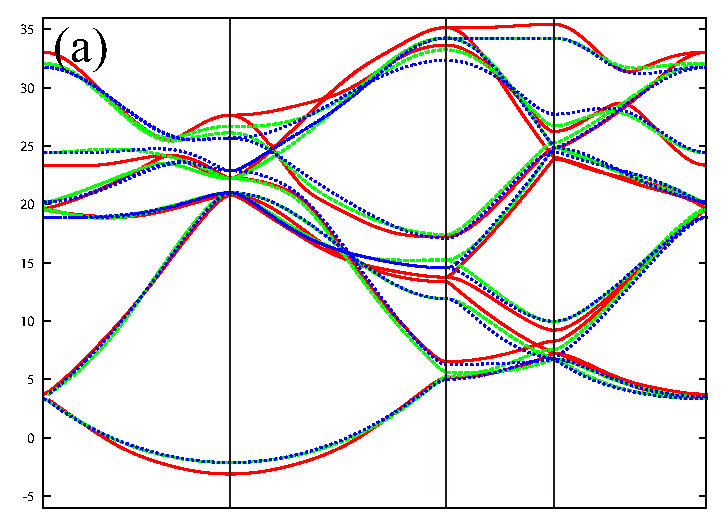
\includegraphics[width=7cm]{band-vs-th.eps}
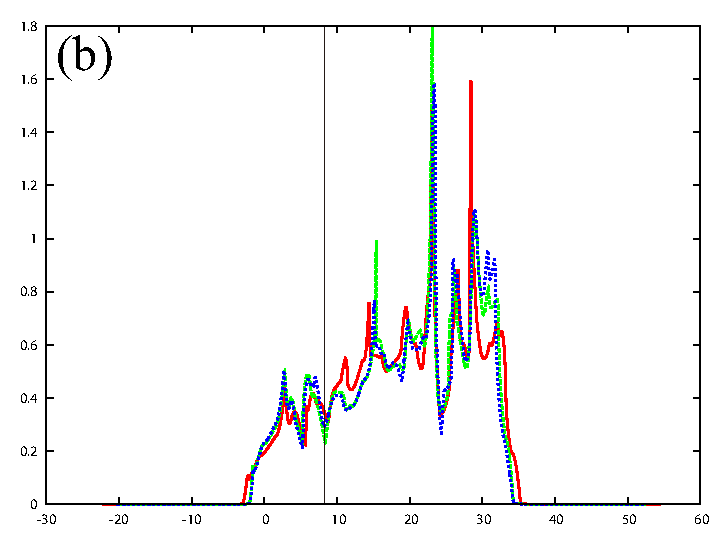
\includegraphics[width=7cm]{dos-vs-th.eps}
\caption{\tr{Energy cutoff dependence on transfer integral: (a) Wannier-interpolated band: \texttt{python tr.py --bnd --ecut=0.0 (red), 0.1 (green), 0.2 (blue)}. (b) Density of states: \texttt{python tr.py --dos --ecut=0.0 (red), 0.1 (green), 0.2 (blue)}.}}
\label{band-dos}
\end{figure}

\vspace{10mm}
\item{K-point grid dependence of the Fermi surface}

\begin{figure}[H] 
\centering
\includegraphics[width=12cm]{frmsf-vs-kgrd.eps}
\caption{\tr{The $k$-grid dependence of the Fermi surface: \texttt{python tr.py --frm --kgrd='8 8 8' (a), '12 12 12' (b), '24 24 24' (c), '48 48 48' (d)}.}}
\label{frmsf}
\end{figure}
\end{itemize}

\clearpage 

\section{\label{La2CuO4}La$_2$CuO$_4$ (Interaction evaluation using constrained RPA)} 

\tr{In this chapter, the evaluation of the interaction parameters of the transition-metal oxide La$_2$CuO$_4$ is described. In particular, we will describe the setting of the inner energy window in {\tt wannier} calculation and the constrained RPA option in {\tt chiqw} calculation. A condition for the band calculation (using {\sc xTAPP}) is a  6$\times$6$\times$6 $k$-point sampling (30 irreducible $k$ points), a wave function cutoff of 81 Ry, the total number of bands of 60 (26 occupied bands, 1 partial occupied band, 33 unoccupied bands, including the bands up to about 15 eV above the Fermi level).} 

\tr{In this calculation, since the constrained RPA calculation is performed, the variable {\tt flg\_cRPA} is set to {\tt 1}. To reduce the computational cost, the polarization function cutoff is set to 3 Ry (8.1 Ry by default). In case of the constrained RPA, we need to perform the {\tt wannier} calculation before the {\tt chiqw} calculation, because exclusion polarization is defined with the Wannier function. Therefore, the order of calculation is {\tt wannier}$\to${\tt chiqw}$\to${\tt calc\_w3d (calc\_j3d)}. Below is {\tt input.in} of La$_2$CuO$_4$ (body centered tetragonal lattice). In this input, the optional parameters are omitted.} 
\vspace{3mm}\hrule
\begin{verbatim}
&param_wannier 
 N_wannier=1,                !Number of Wannier functions you want to calculate
 Lower_energy_window=10.0d0, !Lower limit of energy window (eV)
 Upper_energy_window=15.6d0, !Upper limit of energy window (eV)
 N_initial_guess=1,          !Number of initial Gaussian
 set_inner_window=T,         !Setting of inner energy window
 Lower_inner_window=12.60d0, !Energy inner window lower limit (eV)
 Upper_inner_window=13.40d0/ !Energy inner window lower limit (eV)
 dx2 0.2d0 0.0d0 0.0d0 0.0d0 !Orbital type, Gaussian width, Gaussian position dx2-y2@Cu
&param_interpolation   
 N_sym_points=6/    !Total number of symmetric k points in calculation lines
 0.000 0.000  0.000 !Symmetric k point; SK_sym_pts(1:3,1); G
 0.000 0.000  0.500 !Symmetric k point; SK_sym_pts(1:3,1); X
 0.250 0.250  0.250 !Symmetric k point; SK_sym_pts(1:3,1); P
 0.000 0.500  0.000 !Symmetric k point; SK_sym_pts(1:3,1); N
 0.000 0.000  0.000 !Symmetric k point; SK_sym_pts(1:3,1); G
 0.500 0.500 -0.500 !Symmetric k point; SK_sym_pts(1:3,1); Z
&param_visualization
 flg_vis_wannier=1/ !Calculate realspace Wannier function (Do not: 0, do 1)   
&param_chiqw 
 Ecut_for_eps=3.0d0, !Cutoff of polarization function (Ry)
 flg_cRPA=1/         !Constrained RPA option (0: RPA, 1: cRPA)
&param_calc_int 
 /
\end{verbatim}
\hrule\vspace{3mm}

In the \verb+wannier+ calculation, we set the energy window to \verb+Lower_energy_ window=10.0 eV+ and \verb+Upper_energy_ window=15.6 eV+. \tr{Note that the values of the energy window depend on the band-calculation software.} We make the Wannier function with initial guess of $d_{x^2-y^2}$ centered at the position of the copper atom (\verb+dx2 0.2d0 0.0d0 0.0d0 0.0d0+). In this calculation, the inner window is set (\verb+set_inner_ window=T+). The inner window is set to \verb+Lower_inner_ window=12.6 eV+ and \verb+Upper_inner_window=13.4 eV+. The bands within the inner window is basically reproduced. The inner window is usually set to sandwich the Fermi level (12.97 eV in this calculation).

\tr{The resulting Wannier-interpolated band and realspace Wannier function are shown in Fig.~\ref{band-La2CuO4} and \ref{vesta-La2CuO4}, respectively. We show the wavenumber dependence of the static inverse dielectric function by constrained RPA and normal RPA for Fig.~\ref{epsqw-cRPA-La2CuO4}~(a) and (b), respectively. We also show the electronic energy loss spectrum (eels) by constrained RPA and normal RPA on Figs~\ref{eels-cRPA-La2CuO4}~(a) and (b), respectively. The distance dependence of the statically screened direct integrals is shown in Fig.~\ref{WvsR-La2CuO4}, where red, green, and blue are bare, constrained-RPA, and normal-RPA direct integrals, respectively. We show the frequency dependence of onsite screened direct integral by constrained RPA and normal RPA for Figs~\ref{UvsE-cRPA-La2CuO4}~(a) and (b), respectively.} 

\begin{figure}[h] 
\centering
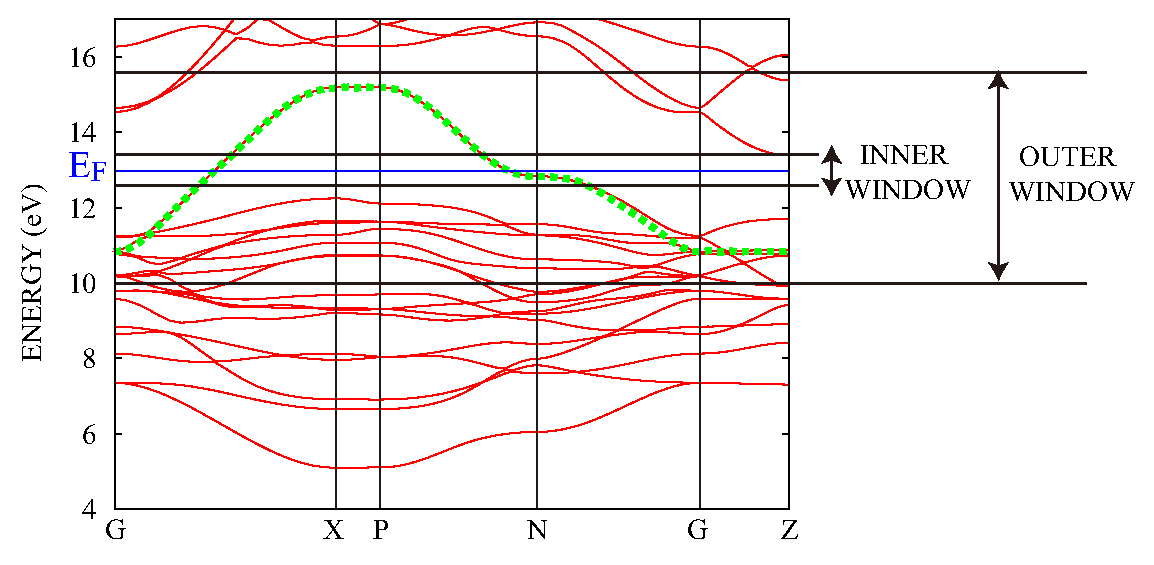
\includegraphics[width=10cm]{dat.iband.La2CuO4.eps}
\caption{Calculated Wannier interpolated band. The unit of the vertical axis is {\tt eV}. The lower limit of the energy window was set to 10 eV ({\tt Lower\_energy\_window=10.0}) and the upper limit was set to 15.6 eV ({\tt Upper\_energy\_window=15.6}). A single Wannier orbital ({\tt N\_wannier=1}) from the bands in this window was made from one initial Gaussian ({\tt N\_initial\_guess=1}). The inner energy window was set to {\tt Lower\_inner\_window=12.6 eV} and {\tt Upper\_inner\_window=13.4 eV}.}
\label{band-La2CuO4}
\end{figure}
\begin{figure}[H] 
\centering
\includegraphics[width=8cm]{dat.wan-realspace-La2CuO4.eps}
\caption{Realspace Wannier function: \tr{The Wannier function data is superposed on the structure data whose size matches the display range of the Wannier function ($2\times2\times2$ supercell).}} 
\label{vesta-La2CuO4}
\end{figure}
\begin{figure}[H] 
\centering
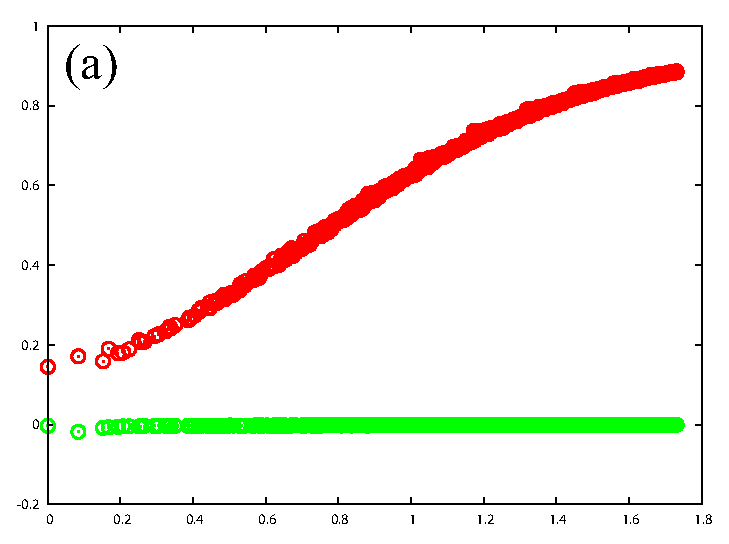
\includegraphics[width=6cm]{epsq0-cRPA-La2CuO4.eps}
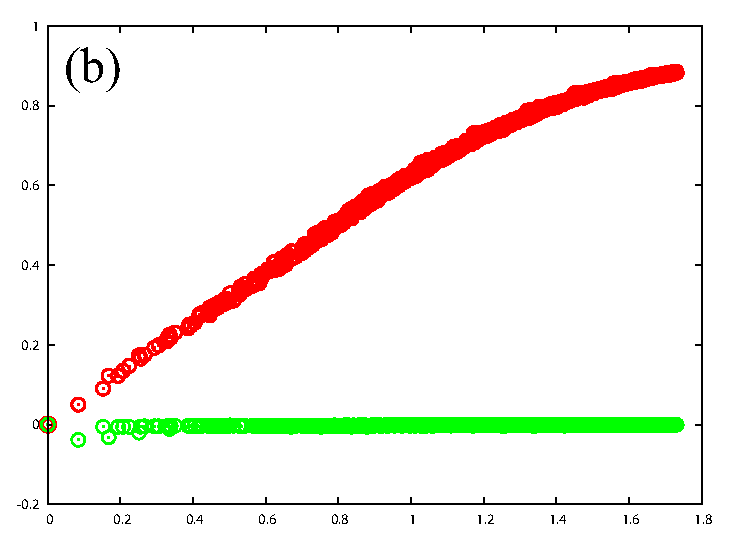
\includegraphics[width=6cm]{epsq0-fRPA-La2CuO4.eps}
\caption{Diagonal data of calculated inverse dielectric matrix with constrained RPA, $\epsilon_{{\bf GG}}^{-1} ({\bf q}, \omega_1)$. (Red is the real part, green is the imaginary part). The horizontal axis is $|{\bf q+G}|$ (bohr $^{- 1}$). The result of $\omega_1=0$ is plotted.}
\label{epsqw-cRPA-La2CuO4}
\end{figure}
\begin{figure}[H] 
\centering
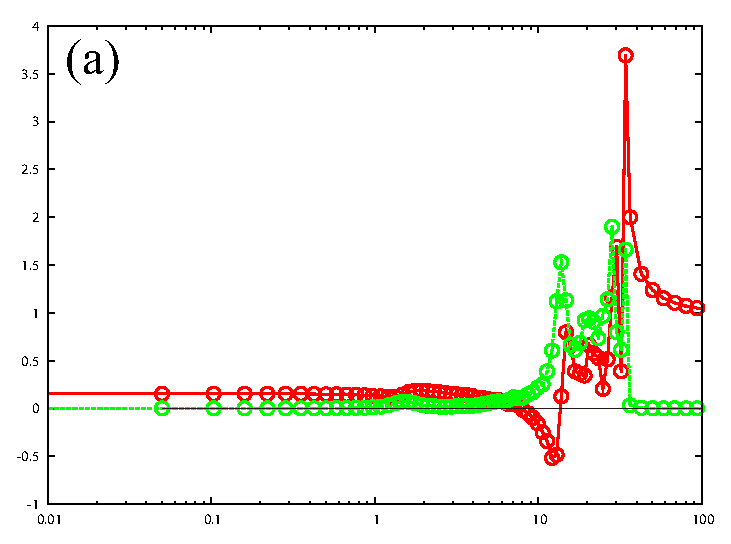
\includegraphics[width=6cm]{eels-cRPA-La2CuO4.eps}
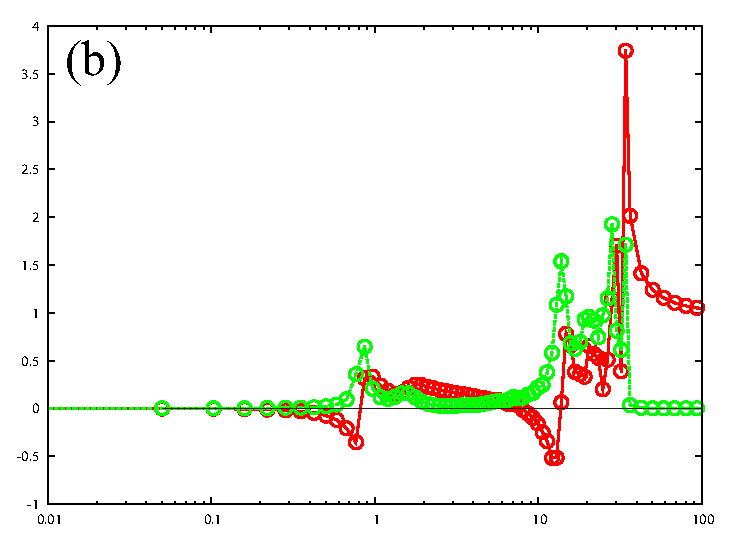
\includegraphics[width=6cm]{eels-fRPA-La2CuO4.eps}
\caption{Calculated eels with constrained RPA [$\epsilon_{{\bf 00}}^{-1}(\Gamma, \omega)$] (red is the real part, green is the imaginary part). The horizontal axis is the logarithm of the frequency $\omega$ (Hartree).}
\label{eels-cRPA-La2CuO4}
\end{figure}
\begin{figure}[H] 
\centering
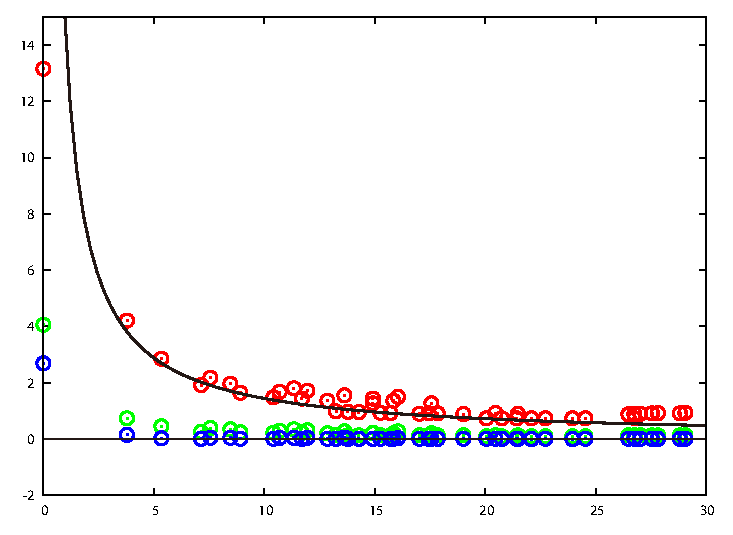
\includegraphics[width=7cm]{WvsR-La2CuO4.eps}
\caption{Distance dependence of direct integral [bare (red), constrained-RPA (green), normal-RPA (blue)]. The horizontal axis is the distance (unit: \AA) between the Wannier functions $w_{i{\bf 0}}$ and $w_{j{\bf R}}$. The unit of the vertical axis is {\tt eV}. Bare direct integral is attenuated with ${\Huge \frac{1}{R}}$. The constrained-RPA direct integral has finite offsite interactions, while the normal-RPA direct integral has the onsite interaction only because of metal screening.}
\label{WvsR-La2CuO4}
\end{figure}
\begin{figure}[H] 
\centering
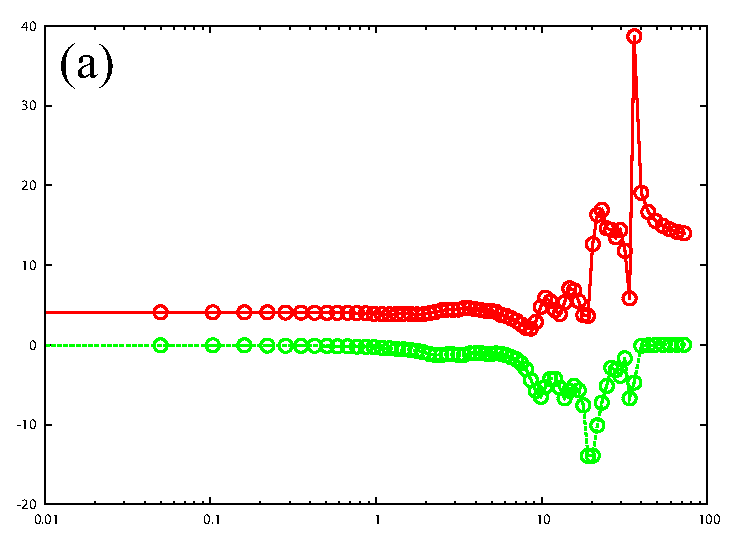
\includegraphics[width=7cm]{UvsE-cRPA-La2CuO4.eps}
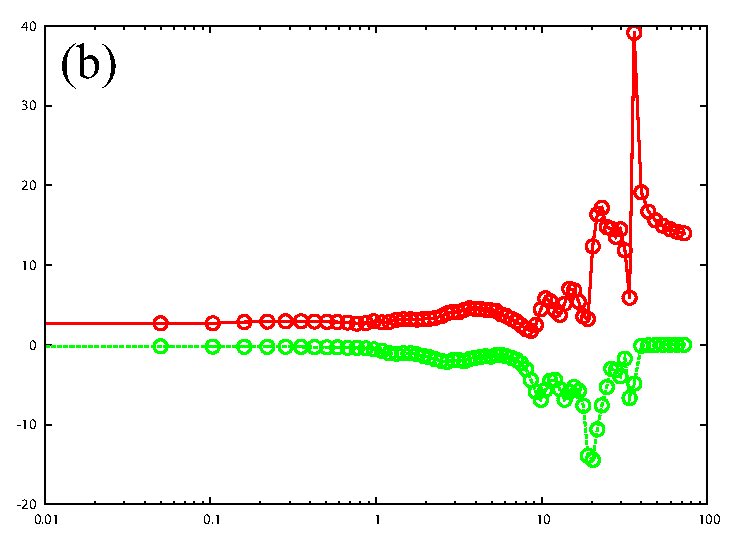
\includegraphics[width=7cm]{UvsE-fRPA-La2CuO4.eps}
\caption{Frequency dependence of onsite screened direct integral with constrained RPA. Red is the real part, and green is the imaginary part. The horizontal axis is the logarithm of the frequency $\omega$ ({\tt eV}). The unit of the vertical axis is {\tt eV}.}
\label{UvsE-cRPA-La2CuO4}
\end{figure}

\clearpage 

\section{\label{TiO2}TiO$_2$ (Wannier function calculation with local coordinates)} 
\tr{We next describe} the calculation to construct the Wannier function by setting the initial Gaussian along the local coordinates. As an example, we consider constructing the $t_{2g}$ Wannier function of TiO$_2$ (rutile structure). The following is \verb+input.in+ for this calculation. The band calculation is preformed using {\sc xTAPP} with $k$-point sampling of 6$\times$6$\times$6 (64 irreducible $k$ points) and 64-Ry wavefunction cutoff. \tr{Note that the values of the energy window in {\tt \&param\_wannier} depend on the band-calculation software.}
\vspace{3mm}\hrule
\begin{verbatim}
&param_wannier 
 N_wannier=6,                !Number of Wannier functions you want to calculate
 LOWER_energy_window= 7.0d0, !Lower limit of energy window (eV)
 UPPER_energy_window=11.0d0, !Upper limit of energy window (eV)
 flg_initial_guess_direc=1,  !Display coordinate of initial Gaussian
 N_initial_guess=6/          !Number of initial Gaussian
 dxy 0.20 0.00 0.00 0.00  0.46 -0.46 0.76 0.46 -0.46 -0.76  0.71 0.71 0.00 !dxy@Ti1
 dyz 0.20 0.00 0.00 0.00  0.46 -0.46 0.76 0.46 -0.46 -0.76  0.71 0.71 0.00 !dyz@Ti1
 dzx 0.20 0.00 0.00 0.00  0.46 -0.46 0.76 0.46 -0.46 -0.76  0.71 0.71 0.00 !dzx@Ti1
 dxy 0.20 0.50 0.50 0.50 -0.46 -0.46 0.76 0.46  0.46  0.76 -0.71 0.71 0.00 !dxy@Ti2
 dyz 0.20 0.50 0.50 0.50 -0.46 -0.46 0.76 0.46  0.46  0.76 -0.71 0.71 0.00 !dyz@Ti2
 dzx 0.20 0.50 0.50 0.50 -0.46 -0.46 0.76 0.46  0.46  0.76 -0.71 0.71 0.00 !dzx@Ti2
&param_interpolation   
 N_sym_points=5/ !Total number of symmetric k points in calculation lines
 0.50 0.00 0.50  !Symmetric k point; SK_sym_pts(1:3,1); M
 0.00 0.00 0.50  !Symmetric k point; SK_sym_pts(1:3,1); Z
 0.00 0.00 0.00  !Symmetric k point; SK_sym_pts(1:3,1); G
 0.50 0.00 0.00  !Symmetric k point; SK_sym_pts(1:3,1); X
 0.00 0.50 0.00  !Symmetric k point; SK_sym_pts(1:3,1); Y
&param_visualization   
 FLG_VIS_WANNIER=1/ !Calculate realspace Wannier function (Do not: 0, do 1)     
\end{verbatim}
\hrule\vspace{3mm}

In this \verb+wannier+ calculation, we set the energy window to \verb+Lower_energy_window=7.0 eV+ and  \verb+Upper_energy_window=11.0 eV+ to include the $t_{2 g}$ bands. Also, in this calculation the variable \verb+flg_initial_guess_direc+ has been set to \verb+1+. As a result, the display coordinate of the initial Gaussian is changed to the local coordinate system. With this flag set, in addition to the basic information of the initial Gaussian, the local coordinate information defining the display coordinates are additionally input. Specifically, it is input as follows.
\vspace{3mm}\hrule
\begin{verbatim}
 dxy 0.20 0.50 0.50 0.50 -0.46 -0.46 0.76  0.46 0.46 0.76  -0.71 0.71 0.00
\end{verbatim}
\hrule\vspace{3mm}
In the above, we place \verb+dxy+ Gaussian with width \verb+0.2 (au)+ at the position of \verb+(0.50, 0.50, 0.50)+ in the lattice coordinates. Also, this Gaussian is displayed along the local coordinates (${\bf L}_x, {\bf L}_y, {\bf L}_z$). Here, each local coordinate is as follows.
\begin{eqnarray} 
{\bf L}_x &=& -0.46 {\bf e}_x -0.46 {\bf e}_y + 0.76 {\bf e}_z, \nonumber \\
{\bf L}_y &=& +0.46 {\bf e}_x +0.46 {\bf e}_y + 0.76 {\bf e}_z, \nonumber \\
{\bf L}_z &=& -0.71 {\bf e}_x +0.71 {\bf e}_y + 0.00 {\bf e}_z, \nonumber 
\end{eqnarray} 
Here, ${\bf e}_x, {\bf e}_y, {\bf e}_z$ represent the Cartesian coordinates which are used in the band calculation. The local coordinates ${\bf L}_x, {\bf L}_y, {\bf L}_z$ are defined on the basis of the TiO$_6$ octahedron unit. ${\bf L}_x, {\bf L}_y, {\bf L}_z$ and ${\ bf e}_x, {\bf e}_y, {\bf e}_z$ are shown in Fig.~\ref{TiO2-local}. Regarding the components of the local coordinates, \tr{the user must calculate the values from the structure information by themselves. In this case, we calculated them from the positions of the Ti atoms and the adjacent O atoms in the TiO$_6$ octahedron unit.} 
\begin{figure}[H] 
\centering
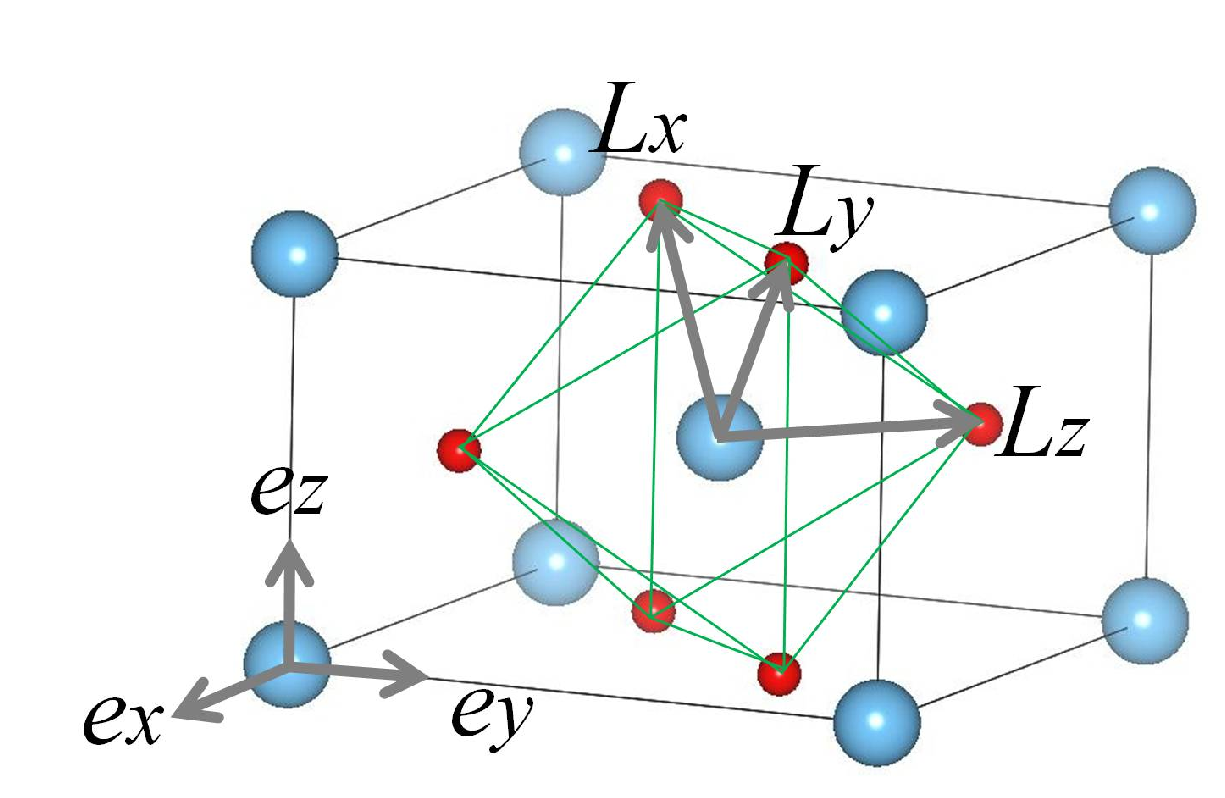
\includegraphics[width=8cm]{TiO2-local.eps}
\caption{Definition of the local coordinates and the Cartesian coordinates in rutile type TiO$_2$. The green frame describes TiO$_6$ octahedron unit.}
\label{TiO2-local}
\end{figure}

Figure~\ref{vesta-TiO2} is the resulting $d_{xy}$-type realspace Wannier function. \tr{It can be seen that the $d_{xy}$ orbital is based on the local coordinates defined by Fig.~\ref{TiO2-local}.} 
\begin{figure}[H] 
\centering
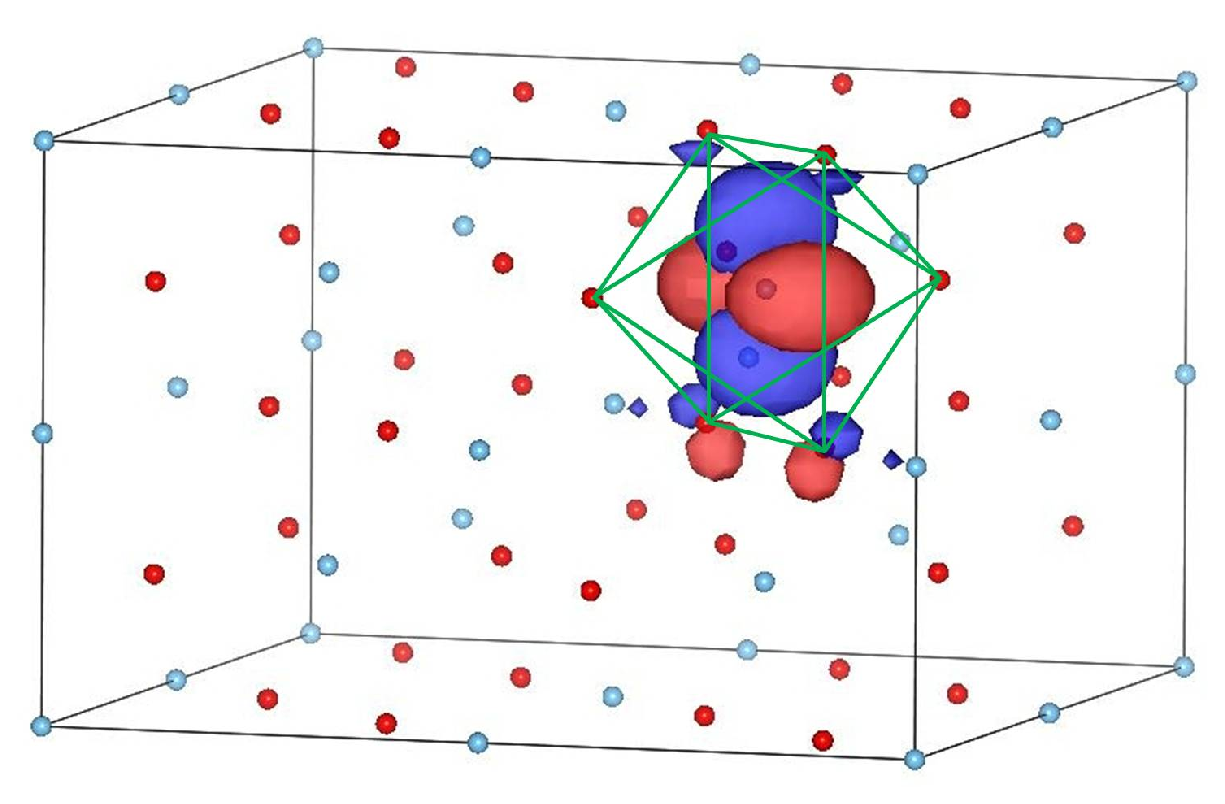
\includegraphics[width=7cm]{dat.wan-realspace-TiO2.eps}
\caption{Calculated realspace $t_{2g}$ Wannier function for rutile TiO$_2$. \tr{The Wannier function data is superposed on the structure data whose size matches the display range of the Wannier function ($2\times2\times2$ supercell).}}
\label{vesta-TiO2}
\end{figure}

\clearpage 

\section{\label{Si}Si (Wannier function using B matrix)} 

\tr{This is an example for constructing the Wannier function by the linear combination of the initial Gaussians.} We consider the Si calculation as an example. The following is \verb+input.in+ for this calculation. The band calculation is preformed using {\sc xTAPP} with $k$-point sampling of 6$\times$6$\times$6 (16 irreducible $k$ points) and 36-Ry wavefunction cutoff. \tr{Note that the values of the energy window in {\tt \&param\_wannier} depend on the band-calculation software.}
\vspace{3mm}\hrule
\begin{verbatim}
&param_wannier 
 N_wannier=8,                  !Lower limit of energy window (eV)
 Upper_energy_window=17.0d0,   !Upper limit of energy window (eV)
 N_initial_guess=8,            !Number of initial Gaussian
 flg_BMAT=1/                   !0:BMAT=unit matrix, 1:reading BMAT      
 s  0.5d0 0.00d0 0.00d0 0.00d0 !s@Si1
 px 0.5d0 0.00d0 0.00d0 0.00d0 !px@Si1
 py 0.5d0 0.00d0 0.00d0 0.00d0 !py@Si1
 pz 0.5d0 0.00d0 0.00d0 0.00d0 !pz@Si1
 s  0.5d0 0.25d0 0.25d0 0.25d0 !s@Si2
 px 0.5d0 0.25d0 0.25d0 0.25d0 !px@Si2
 py 0.5d0 0.25d0 0.25d0 0.25d0 !py@Si2
 pz 0.5d0 0.25d0 0.25d0 0.25d0 !pz@Si2
 0.50 -0.50  0.50 -0.50 0.00  0.00  0.00  0.00 !B_MAT(ig=1,iw=1:8)
 0.50  0.50 -0.50 -0.50 0.00  0.00  0.00  0.00 !B_MAT(ig=2,iw=1:8)
 0.50 -0.50 -0.50  0.50 0.00  0.00  0.00  0.00 !B_MAT(ig=3,iw=1:8)
 0.50  0.50  0.50  0.50 0.00  0.00  0.00  0.00 !B_MAT(ig=4,iw=1:8)
 0.00  0.00  0.00  0.00 0.50  0.50 -0.50  0.50 !B_MAT(ig=5,iw=1:8)
 0.00  0.00  0.00  0.00 0.50 -0.50  0.50  0.50 !B_MAT(ig=6,iw=1:8)
 0.00  0.00  0.00  0.00 0.50  0.50  0.50 -0.50 !B_MAT(ig=7,iw=1:8)
 0.00  0.00  0.00  0.00 0.50 -0.50 -0.50 -0.50 !B_MAT(ig=8,iw=1:8)
&param_interpolation   
 N_sym_points=5/   !Total number of symmetric k points in calculation lines
 0.500 0.500 0.500 !Symmetric k point; SK_sym_pts(1:3,1); L
 0.000 0.000 0.000 !Symmetric k point; SK_sym_pts(1:3,1); G
 0.500 0.000 0.500 !Symmetric k point; SK_sym_pts(1:3,1); X
 0.500 0.250 0.750 !Symmetric k point; SK_sym_pts(1:3,1); W
 0.500 0.500 0.500 !Symmetric k point; SK_sym_pts(1:3,1); L
&param_visualization   
 flg_vis_wannier=1/ !Calculate realspace Wannier function (Do not: 0, do 1)  
\end{verbatim}
\hrule\vspace{3mm}

In this calculation, eight $sp^3$-type Wannier functions of Si are constructed from a linear combination of eight $s$-type and $p$-type Gaussian functions. The B matrix information which are the coefficient of the linear combination is input, \tr{following the initial Gaussian information (look at the part with {\tt B\_MAT} tag). For the B matrix component, the user must calculate the values from the structure information by themselves.} In this case, the components were calculated from the direction along the covalent bond of Si. The size of the B matrix is 8$\times$8, with rows representing the sequence of Gaussian functions and columns representing the sequence of the Wannier orbitals. The component $B_{ij}$ of the B matrix is defined as follows.
\begin{eqnarray}
w_{j}^{in}({\bf r})=\sum_{i}B_{ij} g_i({\bf r}). \nonumber 
\end{eqnarray} 
Here, $g_i$ is the $i$th Gaussian function and $w_{j}^{in}$ is the initial guess of the $j$th Wannier function. The input format of B matrix is as follows. 
\vspace{3mm}\hrule
\begin{verbatim}
do ig=1,N_initial_guess 
 read(5,*) (B_MAT(ig,iw),iw=1,N_wannier) !real(8)
enddo
\end{verbatim}
\hrule\vspace{3mm}
If you set \verb+reading_bmat_format=1+, you can switch in rows and columns of the B matrix. In this case, the row is the Wannier function and the column is the Gaussian function.
\vspace{3mm}\hrule
\begin{verbatim}
do iw=1,N_wannier
 read(5,*) (B_MAT(ig,iw),iw=1,N_initial_guess)
enddo
\end{verbatim}
\hrule\vspace{3mm}
We show calculated $sp^3$-type realspace Wannier function in Fig.~\ref{vesta-Si}.
\begin{figure}[H] 
\centering
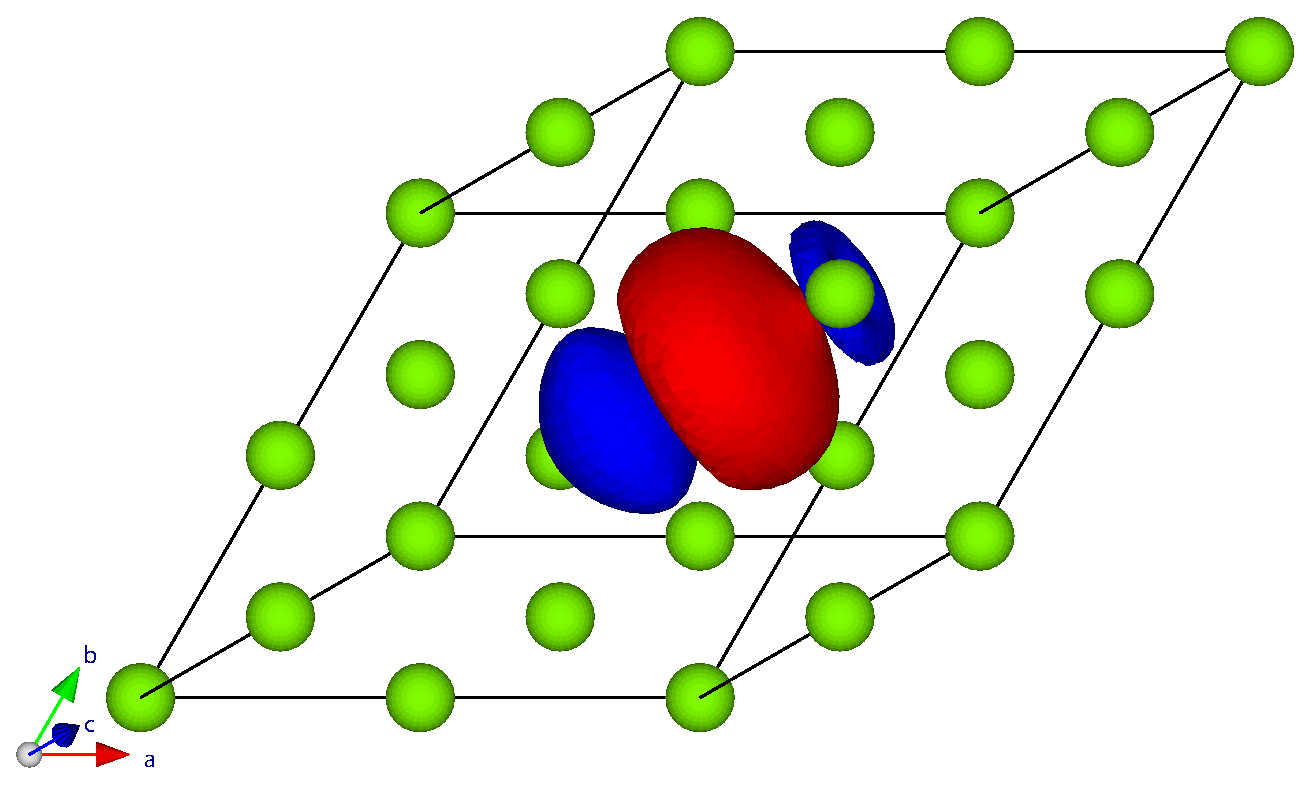
\includegraphics[width=10cm]{dat.wan-realspace-Si.eps}
\caption{Calculated realspace $sp^3$-type Wannier function of Si. \tr{The Wannier function data is superposed on the structure data whose size matches the display range of the Wannier function ($2\times2\times2$ supercell).}}
\label{vesta-Si}
\end{figure}

\clearpage 

\section{\label{SrVO3}SrVO$_3$ (Interaction evaluation using constrained RPA)} 

Below is the input for computing \tr{the interaction parameters} of the $t_{2g}$ Wannier functions of SrVO$_3$ using constrained RPA.
\vspace{3mm}\hrule
\begin{verbatim}
&param_wannier 
 N_wannier=3,                  !Number of Wannier functions you want to calculate
 Lower_energy_window=6.5d0,    !Lower limit of energy window (eV)
 Upper_energy_window=9.7d0,    !Upper limit of energy window (eV)
 N_initial_guess=3/            !Number of initial Gaussian
 dxy 0.5d0 0.5d0  0.5d0  0.5d0 !dxy@V
 dyz 0.5d0 0.5d0  0.5d0  0.5d0 !dyz@V
 dzx 0.5d0 0.5d0  0.5d0  0.5d0 !dzx@V
&param_interpolation   
 N_sym_points=5/   !Total number of symmetric k points in calculation lines
 0.500 0.500 0.500 !Symmetric k point; SK_sym_pts(1:3,1); R 
 0.000 0.000 0.000 !Symmetric k point; SK_sym_pts(1:3,1); G 
 0.500 0.000 0.000 !Symmetric k point; SK_sym_pts(1:3,1); X 
 0.500 0.500 0.000 !Symmetric k point; SK_sym_pts(1:3,1); M 
 0.000 0.000 0.000 !Symmetric k point; SK_sym_pts(1:3,1); G 
&param_visualization   
 / 
&param_chiqw
 Ecut_for_eps=5.0d0,!Cutoff of polarization function (Ry)
 flg_cRPA=1/        !Constrained RPA option (0: normal RPA, 1: constrained RPA)
&param_calc_int 
 /
\end{verbatim}
\hrule\vspace{3mm}
\tr{The band calculation is preformed using {\sc xTAPP} with $k$-point sampling of 6$\times$6$\times$6 (20 irreducible $k$ points), 81-Ry wavefunction cutoff. The total number of bands is 50. Note that the values of the energy window in {\tt \&param\_wannier} depend on the band-calculation software. The condition of the band calculation is loose. If you want convergence, it is better to take 10$times$10$\times$10 $k$ points, 100-Ry wavefunction cutoff, 15-Ry dielectric function cutoff, total number of bands around 100. As SrVO$_3$ has more than one plasmon excitation, it is better to keep the frequency grid as dense as possible. Specifically, it is advisable to set {\tt Num\_freq\_grid=150}. Note that the transition metal has a strong localization and the quantitative accuracy of the interaction parameters may be affected by the pseudopotential. It is better to use a pseudopotential that is as stiff as possible (see Chapter~\ref{pseudopotential}).}  

\clearpage 

\section{\label{TMTSF}(TMTSF)$_2$PF$_6$ (Interaction evaluation using constrained RPA))} 
Below is the input for calculating \tr{the interaction parameters} of an organic compound (TMTSF)$_2$PF$_6$ using constrained RPA. \tr{As the Wannier function, we made HOMO-type orbital localized in organic molecules. The calculations were carried out in System B of Institute for Solid State Physics. It is a parallel job of 72 MPI processes; there are 12 communities and each community has 6 MPI processes. Also, 1 MPI consists of 24 threads. The calculation time was about 100 minutes. {\sc xTAPP} was used for the band calculation. Note that the values of the energy window in {\tt \&param\_wannier} depend on the band-calculation software.}
\vspace{3mm}\hrule
\begin{verbatim}
&param_wannier 
 N_wannier=2,                    !Number of Wannier functions you want to calculate
 Lower_energy_window=2.7d0,      !ƒGLower limit of energy window (eV)
 Upper_energy_window=4.5d0,      !Upper limit of energy window (eV)
 FLG_BMAT=1,                     !0:BMAT=unit matrix, 1:reading BMAT    
 N_initial_guess=6/              !Number of initial Gaussian
 px 0.20 0.26635 0.45950 0.44800 !px@central site of TMTSF molecule #1
 py 0.20 0.26635 0.45950 0.44800 !py@central site of TMTSF molecule #1
 pz 0.20 0.26635 0.45950 0.44800 !pz@central site of TMTSF molecule #1
 px 0.20 0.73365 0.54050 0.55200 !px@central site of TMTSF molecule #2
 py 0.20 0.73365 0.54050 0.55200 !py@central site of TMTSF molecule #2
 0.9995851478  0.0000000000      !B_MAT(ig=1,iw=1:2)
 0.0012540916  0.0000000000      !B_MAT(ig=2,iw=1:2)
-0.0287742877  0.0000000000      !B_MAT(ig=3,iw=1:2)
 0.0000000000  0.9996715835      !B_MAT(ig=4,iw=1:2)
 0.0000000000 -0.0140153561      !B_MAT(ig=5,iw=1:2)
 0.0000000000 -0.0214544857      !B_MAT(ig=6,iw=1:2)
&param_interpolation   
 N_sym_points=5/   !Total number of symmetric k points in calculation lines
 0.000 0.500 0.000 !Symmetric k point; SK_sym_pts(1:3,1); Y
 0.000 0.000 0.000 !Symmetric k point; SK_sym_pts(1:3,1); G
 0.500 0.000 0.000 !Symmetric k point; SK_sym_pts(1:3,1); X
 0.500 0.500 0.000 !Symmetric k point; SK_sym_pts(1:3,1); M 
 0.000 0.000 0.000 !Symmetric k point; SK_sym_pts(1:3,1); G
&param_visualization   
 /
&param_chiqw 
 flg_cRPA=1,       !Constrained RPA option (0: normal RPA, 1: constrained RPA)
 MPI_num_qcomm=12/ !Total number of MPI communities
&param_calc_int 
 /
\end{verbatim}\hrule

\clearpage 

\section{\label{qcom}\tr{Parallel calculation for q points (chiqw)}}
\tr{Polarization calculations can be parallelized for $q$ points. Consider the case where the total number of MPI processes is 64, the parallel degree for the $q$ points is 4, and the total number of the calculation $q$ points is 20. The parallel degree on the $q$ points is specified with the variable {\tt MPI\_num\_qcomm} in {\tt \&param\_chiqw}. If this variable is 4, all the 64 MPI processes are divided into 4 communities, and each community consists of 16 MPI processes (Fig.~\ref{qcommunity}). Since the total number of the $q$ points is 20, one community performs the polarization calculation for five $q$ points.} 
\vspace{3mm}\hrule
\begin{verbatim}
&param_chiqw 
MPI_num_qcomm=4,           !Total number of MPI communities
MPI_num_proc_per_qcomm=16, !Total MPI per community 
\end{verbatim}
\hrule\vspace{3mm}
\tr{The job is executed as follows. The input command in sh system is as follows. Below, {\tt -np 64} is an instruction to use the 64 MPI processes. Note that this specification differs depending on the processing system and/or machine. In RESPACK, when the total number of the MPI processes ({\tt np}) is divided by {\tt MPI\_num\_qcomm}, if the remainder is not zero, the program is stopped.}  
\vspace{3mm}\hrule
\begin{verbatim}
export OMP_NUM_THREADS=16
export MKL_NUM_THREADS=16
mpirun -np 64 ./calc_chiqw < input.in > LOG.chiqw  
\end{verbatim}
\hrule\vspace{3mm}
\begin{figure}[H] 
\centering
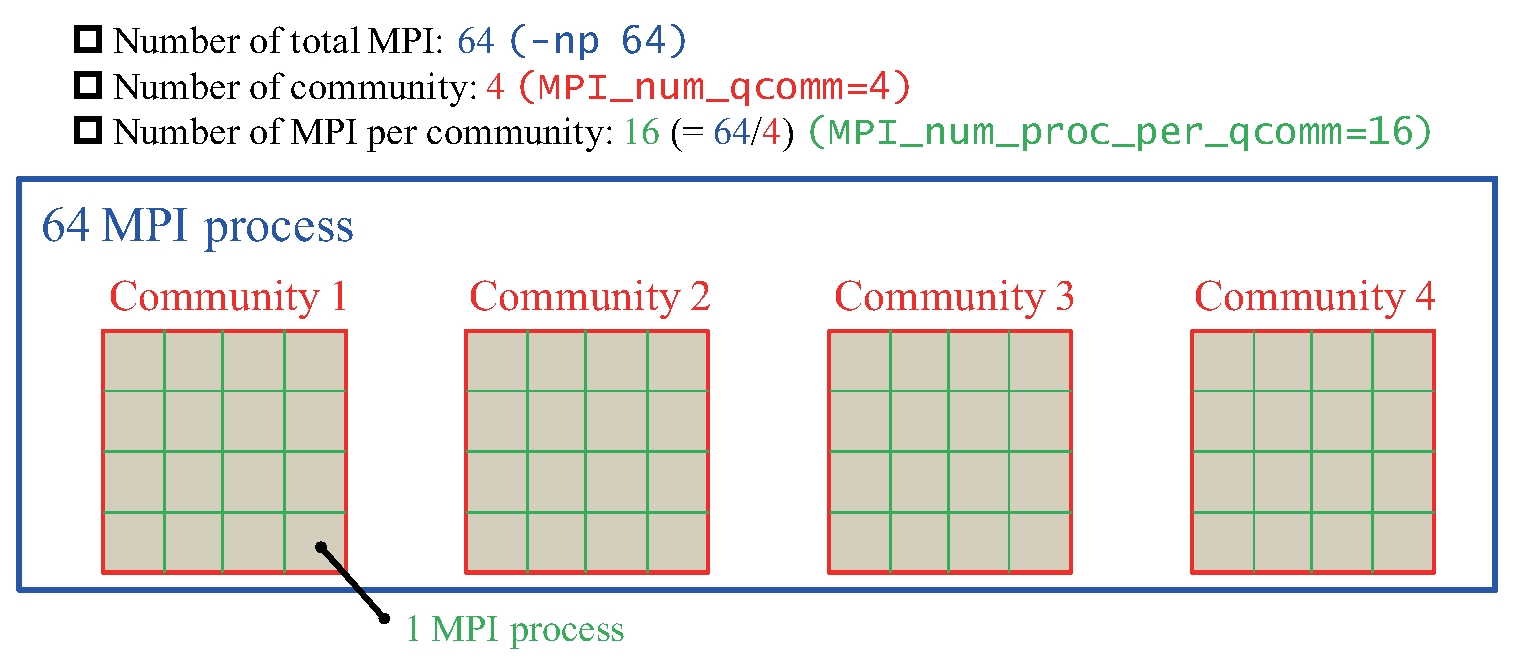
\includegraphics[width=14cm]{q-community.eps}
\caption{\tr{Schematic diagram of parallel computation on $q$ points (the total number of MPI processes {\tt np} is 64). By setting the $q$-point parallel degree to 4 {\tt MPI\_num\_qcomm=4}, all the MPI processes are divided into 4 MPI communities. Each MPI community consists of 16 MPI processes. In RESPACK, when dividing the total number of MPI processes ({\tt np}) by {\tt MPI\_num\_qcomm}, if the remainder is not zero, the program is stopped.}}
\label{qcommunity}
\end{figure}

\clearpage

\section{\label{bulkjob}\tr{Chiqw calculation for specific q points}} 

\tr{Below is the input for executing the {\tt chiqw} calculation for specific $q$ points. In this case, we set the variable {\tt flg\_calc\_type=2} and give the number of the $q$ points we want to calculate ({\tt n\_calc\_q=5}). Then, below the namelist, we specify the numbers of $q$ points we want to compute; {\tt 4 8 14 22 27}. Note that this number is along the sequence of the {\tt dat.sample-k} which contains irreducible $k$ points. In this example, the five $q$ points 4, 8, 14, 22, and 27 are calculated.} 
\vspace{3mm}\hrule
\begin{verbatim}
&param_chiqw 
 flg_calc_type=2, !0:all-q-calc, 1:gamma-only, 2:bulkjob mode 
 n_calc_q=5/      !Total number of q points to calculate
 4 8 14 22 27     !Numbers of q points to be calculated
\end{verbatim}
\hrule\vspace{3mm}

\clearpage 

\section{\label{select-wannier}\tr{Visualization for specific realspace Wannier orbitals}} 

\tr{Below is the input for executing the visualization calculation for specific realspace Wannier functions. In this case, in the namelist {\tt \&param\_visualization}, we give the number of the Wannier functions we want to visualize (in this example, {\tt N\_write\_wannier=3}). Then, below the namelist, we list the numbers of the Wannier functions we want to visualize. In this example, the 1st, 5th and 8th Wannier functions are visualized.} 

\vspace{3mm}\hrule
\begin{verbatim}
&param_visualization 
 N_write_wannier=3/ !Number of realspace Wannier functions you want to calculate
 1 5 8              !Number of the realspace Wannier function you want to calculate
\end{verbatim}
\hrule\vspace{3mm}

\clearpage 

\section{\label{pseudopotential}\tr{Pseudopotential dependence of interaction parameters}} 

\tr{As an example, consider the pseudopotential dependence of the interaction parameter of SrVO$_3$. The pseudopotential depends on the local potential cutoff parameter $r_c$. The pseudopotential constructed with small $r_c$ becomes deeper one, and the pseudo wavefunction obtained with this pseudopotential tends to distribute near the ion core. Figure~\ref{pwn-vs-aewn} compares the pseudo wavefunctions with different cutoff $r_c$ with the all-electron wavefunction (black thick line) for a vanadium atom. As the $r_c$ is reduced to 2.1 \AA (blue line) $\to$ 1.8 \AA (green line) $\to$ 1.5 \AA (red line), the maximum amplitude position of the pseudo wavefunction is shifted to the ion-core side. This tendency is noticeable in orbitals without nodes like the $1s$, $2p$, and $3d$ orbitals. The pseudopotentials with $r_c$ = 1.8 \AA and 2.1 \AA are ionized valence configurations ($3d^{3}4s^{0}4p^{0}$), and the pseudopotential with $r_c$ = 1.5 \AA was created for the ionized semicore configuration ($3s^{2}3p^{6}3d^{3}$). Also, the Troullier-Martins (TM) type was adopted as a function form of the pseudo wavefunction.} 
\begin{figure}[H] 
\centering
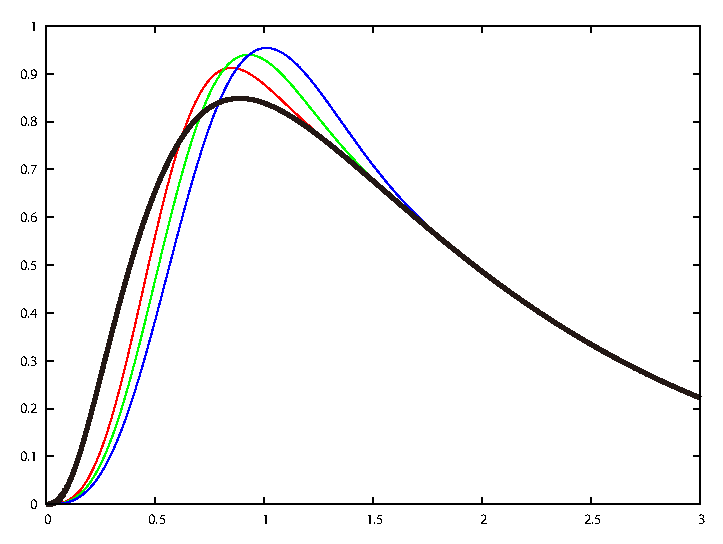
\includegraphics[width=7cm]{pwn_vs_aewn_V.eps}
\caption{\tr{Comparison of the radial part of the pseudo wavefunction and the all-electron wavefunction (black thick line) of the $3d$ orbital of a vanadium atom. The figure shows that, as the local potential cutoff parameter $r_c$ changes to 1.5 \AA (red line), 1.8 \AA (green line), 2.1 \AA (blue line), how the resulting pseudo wavefunction changes. The horizontal axis is the distance $r$ (\AA). By reducing the $r_c$ parameter, the maximum amplitude position of the pseudo wavefunction is shifted to the ion-core side ($r=0$).}} 
\label{pwn-vs-aewn}
\end{figure}

\tr{This tendency can also be seen in the Wannier function. The Wannier function with a pseudopotential with a small $r_c$ tends to be more localized. As a result, it gives a large direct integral. Table~\ref{rc-vs-interaction} is the $r_c$ dependence of interaction parameters for the $t_{2g}$ Wannier function of SrVO$_3$. The calculation conditions are a $6\times6\times6$ $k$-point sampling, a wavefunction cutoff of 144 Ry. Dielectric-function cutoff is 5 Ry, and the total number of bands is 100.}
We see from the table that $r_c$ and the Wannier spread $\Omega$ has positive correlation, where $\Omega$ is defined as 
\begin{eqnarray}
\Omega=\sqrt{ \langle r^2 \rangle - |\langle \mathbf{r} \rangle|^2 }. \nonumber 
\end{eqnarray}
\tr{It can also be seen that the $r_c$ and onsite direct integrals $U$, $U'$ have a negative correlation. There is no noticeable effect on the exchange integral $J$ and the nearest neighbor direct integral $V$. As pseudopotentials, besides the TM type, there are the RRKJ (Rappe-Rabe-Kaxiras-Joannopoulos) type and the ONCV (Optimized Norm-Conserving Vanderbilt) type. Even if the same cutoff $r_c$ is employed, the results can be quantitatively different due to the difference in the functional form of the pseudopotential, so be careful.} 
\begin{table}[H] 
\begin{center}
\caption{\tr{Pseudopotential dependence of interaction parameters of SrVO$_3$. ``bare" and ``cRPA" represent bare and screened Coulomb interactions. $U$, $U'$, $J$, and $V$ are onsite intraorbital direct integral, onsite interorbital direct integral, onsite exchange integral, and nearest intraobital direct integral, respectively. The unit of the local potential cutoff $r_c$ in the pseudopotential and the Wannier spread $\Omega$ are \AA. The unit of interaction is eV.}}  
\label{rc-vs-interaction}
\vspace{0.3cm} 
\begin{tabular}{c c@{\ \ \ } c@{\ } c@{\ } c@{\ } c@{\ } c@{\ \ } c@{\ }c@{\ }c@{\ }c@{\ }} \hline \hline  \\ [-10pt]  
  -          &      -    &  \multicolumn{4}{c}{bare}   &  &   \multicolumn{4}{c}{cRPA}   \\ \hline \\ [-10pt]  
 $r_c$  & $\Omega$ &  $U$ &   $U'$ &  $J$ &  $V$ &  &   $U$ &   $U'$ &  $J$ &  $V$ \\ \hline \\ [-10pt] 
 1.5    &   1.354  & 15.86 & 14.60  & 0.59 & 3.74 &  &  3.65 &  2.49  & 0.56 & 0.67 \\ 
 1.8    &   1.377  & 15.54 & 14.26  & 0.60 & 3.74 &  &  3.54 &  2.36  & 0.57 & 0.70 \\ 
 2.1    &   1.382  & 15.15 & 13.87  & 0.60 & 3.74 &  &  3.50 &  2.32  & 0.57 & 0.72 \\  \hline \hline
\end{tabular} 
\end{center}
\end{table} 

\clearpage 

\section{\label{fileformat}File format (reading format)} 

\begin{enumerate}
\item \verb+dat.bandcalc+ (Band calculation information)
\begin{verbatim}
OPEN(117,FILE='./dir-wfn/dat.bandcalc') 
read(117,*) Ecut_for_psi !Wavefunction cutoff energy (Ry) real(8)
read(117,*) FermiEnergy  !Fermi energy (au) real(8)
read(117,*) Etot         !Total energy (au) real(8) 
\end{verbatim}
\item \verb+dat.sample-k+ [Sample k point vector (irreducible k point)] 
\begin{verbatim}
OPEN(101,FILE='./dir-wfn/dat.sample-k') 
read(101,*) Nk_irr !Total number of irreducible k point integer
do ik=1,Nk_irr 
 read(101,*) (SKI(i,ik),i=1,3) !Irreducible k point vector real(8)
enddo 
\end{verbatim}
\item \verb+dat.eigenvalue+ [Band energy (irrelevant k points)]
\begin{verbatim}
OPEN(111,FILE='./dir-wfn/dat.eigenvalue') 
rewind(111)
read(111,*) NBAND !Number of bands
do ik=1,Nk_irr 
 do ib=1,NBAND 
  read(111,*) E_EIGI(ib,ik) !Band energy (au) (au) real(8)
 enddo 
enddo      
\end{verbatim}
\item \verb+dat.nkm+ [Expanded G number (irreducible k point)]
]
\begin{verbatim}
OPEN(132,FILE='./dir-wfn/dat.nkm-nw') 
rewind(132)
do ik=1,Nk_irr 
 read(132,*) NGI(ik) !Expanded G number integer
enddo  
\end{verbatim}
\item \verb+dat.kg+ [Expanded G vector (irreducible k point)]
\begin{verbatim}
OPEN(104,FILE='./dir-wfn/dat.kg')
do ik=1,Nk_irr 
 read(104,*) NG_for_psi !Expansion G number at ik point integer
 do ig=1,NG_for_psi 
  read(104,*) (KGI(i,ig,ik),i=1,3) !Expansion G vector at irreducible ik point integer
 enddo 
enddo 
\end{verbatim}
 
\vspace{3cm}

\item \verb+dat.wfn+ [Wavefunction (irreducible k point)] 
\begin{verbatim}
OPEN(102,FILE='./dir-wfn/dat.wfn',FORM='unformatted') 
read(102) ncomp !Number of components
do ik=1,Nk_irr  
 do ib=1,NBAND
  read(102)((C0(ic,i,ib,ik),ic=1,ncomp),i=1,NGI(ik))!Wave function complex (8)
 enddo 
enddo
!In the current version, only ncomp = 1 is supported

\end{verbatim}
\item \verb+dat.lattice+ (Lattice vector)
\begin{verbatim}
OPEN(105,FILE='./dir-wfn/dat.lattice') 
read(105,*) a1(1), a1(2), a1(3) !a1 vector in bohr units real(8)
read(105,*) a2(1), a2(2), a2(3) !a2 vector in bohr units real(8) 
read(105,*) a3(1), a3(2), a3(3) !a3 vector in bohr units real(8) 
\end{verbatim}
\item \verb+dat.symmetry+ (Symmetry, ++Expression that works in inverse space++)
\begin{verbatim}
OPEN(100,FILE='./dir-wfn/dat.symmetry') 
read(100,*) nsymq !Number of symmetry operation integer
read(100,*) nnp   !Partial translation integer
do iop=1,nsymq 
 read(100,*) ((rg(i,j,iop),i=1,3),j=1,3) !Rotation symmetry integer
 read(100,*) (pg(i,iop),i=1,3)           !Partial translational symmetry integer 
enddo 
\end{verbatim}
\item \tr{{\tt dat.atom\_position} (Atomic position)}
\begin{verbatim}
OPEN(108,FILE='./dir-wfn/dat.atom_position')
read(108,*) nsi !Number of atoms
do i=1,nsi
 read(108,*) chemical_species(i), !Atomic species character
+            (asi(j,i),j=1,3)     !Atomic position real(8)
enddo
\end{verbatim}
\end{enumerate}

\clearpage 

\section{\label{license}License} 

\tr{The source codes and utility programs and scripts of this software are distributed on the basis of GNU General Public License version 3 (GPL v3)}.

\section{\label{howtocite}How to quote} 

When quoting RESPACK, it would be appreciated if you could quote the following papers: 
\begin{enumerate} 
\item K. Nakamura, Y. Nohara, Y. Yoshimoto, Y. Nomura, Phys. Rev. B {\bf 93}, 085124 (2016).
\item K. Nakamura, Y. Yoshimoto, T. Kosugi, R. Arita, M. Imada, J. Phys. Soc. Jpn {\bf 78}, 083710 (2009).
\item K. Nakamura, R. Arita, M. Imada, J. Phys. Soc. Jpn {\bf 77}, 093711 (2008).
\item Y. Nohara, S. Yamamoto, T. Fujiwara, Phys. Rev. B {\bf 79}, 195110 (2009).
\item T. Fujiwara, S. Yamamoto, Y. Ishii, J. Phys. Soc. Jpn. {\bf 72}, 777 (2003).
\end{enumerate} 

\end{document}
